% Options for packages loaded elsewhere
\PassOptionsToPackage{unicode}{hyperref}
\PassOptionsToPackage{hyphens}{url}
\PassOptionsToPackage{dvipsnames,svgnames,x11names}{xcolor}
%
\documentclass[
  11pt,
  letterpaper,
  DIV=11,
  numbers=noendperiod]{scrartcl}

\usepackage{amsmath,amssymb}
\usepackage{setspace}
\usepackage{iftex}
\ifPDFTeX
  \usepackage[T1]{fontenc}
  \usepackage[utf8]{inputenc}
  \usepackage{textcomp} % provide euro and other symbols
\else % if luatex or xetex
  \usepackage{unicode-math}
  \defaultfontfeatures{Scale=MatchLowercase}
  \defaultfontfeatures[\rmfamily]{Ligatures=TeX,Scale=1}
\fi
\usepackage{lmodern}
\ifPDFTeX\else  
    % xetex/luatex font selection
\fi
% Use upquote if available, for straight quotes in verbatim environments
\IfFileExists{upquote.sty}{\usepackage{upquote}}{}
\IfFileExists{microtype.sty}{% use microtype if available
  \usepackage[]{microtype}
  \UseMicrotypeSet[protrusion]{basicmath} % disable protrusion for tt fonts
}{}
\makeatletter
\@ifundefined{KOMAClassName}{% if non-KOMA class
  \IfFileExists{parskip.sty}{%
    \usepackage{parskip}
  }{% else
    \setlength{\parindent}{0pt}
    \setlength{\parskip}{6pt plus 2pt minus 1pt}}
}{% if KOMA class
  \KOMAoptions{parskip=half}}
\makeatother
\usepackage{xcolor}
\usepackage[margin = 1in]{geometry}
\setlength{\emergencystretch}{3em} % prevent overfull lines
\setcounter{secnumdepth}{-\maxdimen} % remove section numbering
% Make \paragraph and \subparagraph free-standing
\makeatletter
\ifx\paragraph\undefined\else
  \let\oldparagraph\paragraph
  \renewcommand{\paragraph}{
    \@ifstar
      \xxxParagraphStar
      \xxxParagraphNoStar
  }
  \newcommand{\xxxParagraphStar}[1]{\oldparagraph*{#1}\mbox{}}
  \newcommand{\xxxParagraphNoStar}[1]{\oldparagraph{#1}\mbox{}}
\fi
\ifx\subparagraph\undefined\else
  \let\oldsubparagraph\subparagraph
  \renewcommand{\subparagraph}{
    \@ifstar
      \xxxSubParagraphStar
      \xxxSubParagraphNoStar
  }
  \newcommand{\xxxSubParagraphStar}[1]{\oldsubparagraph*{#1}\mbox{}}
  \newcommand{\xxxSubParagraphNoStar}[1]{\oldsubparagraph{#1}\mbox{}}
\fi
\makeatother

\usepackage{color}
\usepackage{fancyvrb}
\newcommand{\VerbBar}{|}
\newcommand{\VERB}{\Verb[commandchars=\\\{\}]}
\DefineVerbatimEnvironment{Highlighting}{Verbatim}{commandchars=\\\{\}}
% Add ',fontsize=\small' for more characters per line
\usepackage{framed}
\definecolor{shadecolor}{RGB}{241,243,245}
\newenvironment{Shaded}{\begin{snugshade}}{\end{snugshade}}
\newcommand{\AlertTok}[1]{\textcolor[rgb]{0.68,0.00,0.00}{#1}}
\newcommand{\AnnotationTok}[1]{\textcolor[rgb]{0.37,0.37,0.37}{#1}}
\newcommand{\AttributeTok}[1]{\textcolor[rgb]{0.40,0.45,0.13}{#1}}
\newcommand{\BaseNTok}[1]{\textcolor[rgb]{0.68,0.00,0.00}{#1}}
\newcommand{\BuiltInTok}[1]{\textcolor[rgb]{0.00,0.23,0.31}{#1}}
\newcommand{\CharTok}[1]{\textcolor[rgb]{0.13,0.47,0.30}{#1}}
\newcommand{\CommentTok}[1]{\textcolor[rgb]{0.37,0.37,0.37}{#1}}
\newcommand{\CommentVarTok}[1]{\textcolor[rgb]{0.37,0.37,0.37}{\textit{#1}}}
\newcommand{\ConstantTok}[1]{\textcolor[rgb]{0.56,0.35,0.01}{#1}}
\newcommand{\ControlFlowTok}[1]{\textcolor[rgb]{0.00,0.23,0.31}{\textbf{#1}}}
\newcommand{\DataTypeTok}[1]{\textcolor[rgb]{0.68,0.00,0.00}{#1}}
\newcommand{\DecValTok}[1]{\textcolor[rgb]{0.68,0.00,0.00}{#1}}
\newcommand{\DocumentationTok}[1]{\textcolor[rgb]{0.37,0.37,0.37}{\textit{#1}}}
\newcommand{\ErrorTok}[1]{\textcolor[rgb]{0.68,0.00,0.00}{#1}}
\newcommand{\ExtensionTok}[1]{\textcolor[rgb]{0.00,0.23,0.31}{#1}}
\newcommand{\FloatTok}[1]{\textcolor[rgb]{0.68,0.00,0.00}{#1}}
\newcommand{\FunctionTok}[1]{\textcolor[rgb]{0.28,0.35,0.67}{#1}}
\newcommand{\ImportTok}[1]{\textcolor[rgb]{0.00,0.46,0.62}{#1}}
\newcommand{\InformationTok}[1]{\textcolor[rgb]{0.37,0.37,0.37}{#1}}
\newcommand{\KeywordTok}[1]{\textcolor[rgb]{0.00,0.23,0.31}{\textbf{#1}}}
\newcommand{\NormalTok}[1]{\textcolor[rgb]{0.00,0.23,0.31}{#1}}
\newcommand{\OperatorTok}[1]{\textcolor[rgb]{0.37,0.37,0.37}{#1}}
\newcommand{\OtherTok}[1]{\textcolor[rgb]{0.00,0.23,0.31}{#1}}
\newcommand{\PreprocessorTok}[1]{\textcolor[rgb]{0.68,0.00,0.00}{#1}}
\newcommand{\RegionMarkerTok}[1]{\textcolor[rgb]{0.00,0.23,0.31}{#1}}
\newcommand{\SpecialCharTok}[1]{\textcolor[rgb]{0.37,0.37,0.37}{#1}}
\newcommand{\SpecialStringTok}[1]{\textcolor[rgb]{0.13,0.47,0.30}{#1}}
\newcommand{\StringTok}[1]{\textcolor[rgb]{0.13,0.47,0.30}{#1}}
\newcommand{\VariableTok}[1]{\textcolor[rgb]{0.07,0.07,0.07}{#1}}
\newcommand{\VerbatimStringTok}[1]{\textcolor[rgb]{0.13,0.47,0.30}{#1}}
\newcommand{\WarningTok}[1]{\textcolor[rgb]{0.37,0.37,0.37}{\textit{#1}}}

\providecommand{\tightlist}{%
  \setlength{\itemsep}{0pt}\setlength{\parskip}{0pt}}\usepackage{longtable,booktabs,array}
\usepackage{calc} % for calculating minipage widths
% Correct order of tables after \paragraph or \subparagraph
\usepackage{etoolbox}
\makeatletter
\patchcmd\longtable{\par}{\if@noskipsec\mbox{}\fi\par}{}{}
\makeatother
% Allow footnotes in longtable head/foot
\IfFileExists{footnotehyper.sty}{\usepackage{footnotehyper}}{\usepackage{footnote}}
\makesavenoteenv{longtable}
\usepackage{graphicx}
\makeatletter
\newsavebox\pandoc@box
\newcommand*\pandocbounded[1]{% scales image to fit in text height/width
  \sbox\pandoc@box{#1}%
  \Gscale@div\@tempa{\textheight}{\dimexpr\ht\pandoc@box+\dp\pandoc@box\relax}%
  \Gscale@div\@tempb{\linewidth}{\wd\pandoc@box}%
  \ifdim\@tempb\p@<\@tempa\p@\let\@tempa\@tempb\fi% select the smaller of both
  \ifdim\@tempa\p@<\p@\scalebox{\@tempa}{\usebox\pandoc@box}%
  \else\usebox{\pandoc@box}%
  \fi%
}
% Set default figure placement to htbp
\def\fps@figure{htbp}
\makeatother

\usepackage{fvextra}
\DefineVerbatimEnvironment{Highlighting}{Verbatim}{breaklines,commandchars=\\\{\}}
\DefineVerbatimEnvironment{OutputCode}{Verbatim}{breaklines,commandchars=\\\{\}}
\KOMAoption{captions}{tableheading}
\makeatletter
\@ifpackageloaded{caption}{}{\usepackage{caption}}
\AtBeginDocument{%
\ifdefined\contentsname
  \renewcommand*\contentsname{Table of contents}
\else
  \newcommand\contentsname{Table of contents}
\fi
\ifdefined\listfigurename
  \renewcommand*\listfigurename{List of Figures}
\else
  \newcommand\listfigurename{List of Figures}
\fi
\ifdefined\listtablename
  \renewcommand*\listtablename{List of Tables}
\else
  \newcommand\listtablename{List of Tables}
\fi
\ifdefined\figurename
  \renewcommand*\figurename{Figure}
\else
  \newcommand\figurename{Figure}
\fi
\ifdefined\tablename
  \renewcommand*\tablename{Table}
\else
  \newcommand\tablename{Table}
\fi
}
\@ifpackageloaded{float}{}{\usepackage{float}}
\floatstyle{ruled}
\@ifundefined{c@chapter}{\newfloat{codelisting}{h}{lop}}{\newfloat{codelisting}{h}{lop}[chapter]}
\floatname{codelisting}{Listing}
\newcommand*\listoflistings{\listof{codelisting}{List of Listings}}
\makeatother
\makeatletter
\makeatother
\makeatletter
\@ifpackageloaded{caption}{}{\usepackage{caption}}
\@ifpackageloaded{subcaption}{}{\usepackage{subcaption}}
\makeatother

\usepackage{bookmark}

\IfFileExists{xurl.sty}{\usepackage{xurl}}{} % add URL line breaks if available
\urlstyle{same} % disable monospaced font for URLs
\hypersetup{
  pdftitle={STATS 3DA3},
  pdfauthor={Yixin Ma (4004285971), Runhan Huang (40047799), Kunhan Liang (400315267)},
  colorlinks=true,
  linkcolor={blue},
  filecolor={Maroon},
  citecolor={Blue},
  urlcolor={Blue},
  pdfcreator={LaTeX via pandoc}}


\title{STATS 3DA3}
\usepackage{etoolbox}
\makeatletter
\providecommand{\subtitle}[1]{% add subtitle to \maketitle
  \apptocmd{\@title}{\par {\large #1 \par}}{}{}
}
\makeatother
\subtitle{Homework Assignment 6}
\author{Yixin Ma (4004285971), Runhan Huang (40047799), Kunhan Liang
(400315267)}
\date{2025-04-13}

\begin{document}
\maketitle


\setstretch{1.5}
\newpage

\begin{Shaded}
\begin{Highlighting}[]
\ImportTok{import}\NormalTok{ pandas }\ImportTok{as}\NormalTok{ pd}
\ImportTok{from}\NormalTok{ sklearn.preprocessing }\ImportTok{import}\NormalTok{ StandardScaler}
\ImportTok{from}\NormalTok{ sklearn.model\_selection }\ImportTok{import}\NormalTok{ train\_test\_split}

\ImportTok{from}\NormalTok{ sklearn.cluster }\ImportTok{import}\NormalTok{ KMeans}
\ImportTok{from}\NormalTok{ sklearn.decomposition }\ImportTok{import}\NormalTok{ PCA}
\ImportTok{from}\NormalTok{ sklearn.metrics }\ImportTok{import}\NormalTok{ silhouette\_score, silhouette\_samples}
\ImportTok{import}\NormalTok{ matplotlib.pyplot }\ImportTok{as}\NormalTok{ plt}
\ImportTok{import}\NormalTok{ matplotlib.cm }\ImportTok{as}\NormalTok{ cm}
\ImportTok{import}\NormalTok{ numpy }\ImportTok{as}\NormalTok{ np}
\ImportTok{import}\NormalTok{ seaborn }\ImportTok{as}\NormalTok{ sns}

\ImportTok{from}\NormalTok{ sklearn.linear\_model }\ImportTok{import}\NormalTok{ LogisticRegression}
\ImportTok{from}\NormalTok{ sklearn.metrics }\ImportTok{import}\NormalTok{ accuracy\_score, confusion\_matrix, classification\_report}

\ImportTok{from}\NormalTok{ sklearn.model\_selection }\ImportTok{import}\NormalTok{ cross\_val\_score}
\ImportTok{from}\NormalTok{ sklearn.tree }\ImportTok{import}\NormalTok{ DecisionTreeClassifier}
\ImportTok{from}\NormalTok{ mlxtend.feature\_selection }\ImportTok{import}\NormalTok{ SequentialFeatureSelector }\ImportTok{as}\NormalTok{ SFS}
\ImportTok{from}\NormalTok{ sklearn.ensemble }\ImportTok{import}\NormalTok{ RandomForestClassifier}
\ImportTok{from}\NormalTok{ sklearn.model\_selection }\ImportTok{import}\NormalTok{ GridSearchCV}
\end{Highlighting}
\end{Shaded}

\begin{enumerate}
\def\labelenumi{(\arabic{enumi})}
\tightlist
\item
\end{enumerate}

A classification problem is to use a set of 13 features to predict
whether a person has heart disease or not.

\begin{enumerate}
\def\labelenumi{(\arabic{enumi})}
\setcounter{enumi}{1}
\tightlist
\item
\end{enumerate}

\begin{Shaded}
\begin{Highlighting}[]
\CommentTok{\# Load the dataset}
\NormalTok{data }\OperatorTok{=}\NormalTok{ pd.read\_csv(}\StringTok{\textquotesingle{}ass6{-}dataset.csv\textquotesingle{}}\NormalTok{)}

\CommentTok{\# Scale the data (excluding the target variable "num")}
\NormalTok{features }\OperatorTok{=}\NormalTok{ data.drop(columns}\OperatorTok{=}\NormalTok{[}\StringTok{\textquotesingle{}num\textquotesingle{}}\NormalTok{])}
\NormalTok{scaler }\OperatorTok{=}\NormalTok{ StandardScaler()}
\NormalTok{scaled\_features }\OperatorTok{=}\NormalTok{ scaler.fit\_transform(features)}
\NormalTok{scaled\_data }\OperatorTok{=}\NormalTok{ pd.DataFrame(scaled\_features, columns}\OperatorTok{=}\NormalTok{features.columns)}
\NormalTok{scaled\_data[}\StringTok{\textquotesingle{}num\textquotesingle{}}\NormalTok{] }\OperatorTok{=}\NormalTok{ data[}\StringTok{\textquotesingle{}num\textquotesingle{}}\NormalTok{]}
\end{Highlighting}
\end{Shaded}

\begin{enumerate}
\def\labelenumi{(\arabic{enumi})}
\setcounter{enumi}{2}
\tightlist
\item
\end{enumerate}

\begin{Shaded}
\begin{Highlighting}[]
\CommentTok{\# Get the list of variables of the dataset}
\NormalTok{variables }\OperatorTok{=}\NormalTok{ data.columns.tolist()}
\BuiltInTok{print}\NormalTok{(}\StringTok{"Variables in the dataset:"}\NormalTok{)}
\ControlFlowTok{for}\NormalTok{ var }\KeywordTok{in}\NormalTok{ variables:}
    \BuiltInTok{print}\NormalTok{(var)}

\CommentTok{\# Get a summary of the dataset}
\NormalTok{summary }\OperatorTok{=}\NormalTok{ data.describe()}
\BuiltInTok{print}\NormalTok{(}\StringTok{"}\CharTok{\textbackslash{}n}\StringTok{Summary of the dataset:"}\NormalTok{)}
\BuiltInTok{print}\NormalTok{(summary)}

\CommentTok{\# Get the number of observations}
\NormalTok{num\_observations }\OperatorTok{=}\NormalTok{ data.shape[}\DecValTok{0}\NormalTok{]}
\BuiltInTok{print}\NormalTok{(}\SpecialStringTok{f"}\CharTok{\textbackslash{}n}\SpecialStringTok{Number of observations: }\SpecialCharTok{\{}\NormalTok{num\_observations}\SpecialCharTok{\}}\SpecialStringTok{"}\NormalTok{)}

\CommentTok{\# Get the data types of the variables}
\NormalTok{data\_types }\OperatorTok{=}\NormalTok{ data.dtypes}
\BuiltInTok{print}\NormalTok{(}\StringTok{"}\CharTok{\textbackslash{}n}\StringTok{Data types of the variables:"}\NormalTok{)}
\BuiltInTok{print}\NormalTok{(data\_types)}

\CommentTok{\# Get the distribution of the variables}
\BuiltInTok{print}\NormalTok{(}\StringTok{"}\CharTok{\textbackslash{}n}\StringTok{Distribution of the variables:"}\NormalTok{)}
\ControlFlowTok{for}\NormalTok{ var }\KeywordTok{in}\NormalTok{ variables:}
    \BuiltInTok{print}\NormalTok{(}\SpecialStringTok{f"}\CharTok{\textbackslash{}n}\SpecialCharTok{\{}\NormalTok{var}\SpecialCharTok{\}}\SpecialStringTok{:"}\NormalTok{)}
    \BuiltInTok{print}\NormalTok{(data[var].value\_counts())}
    \BuiltInTok{print}\NormalTok{(data[var].describe())}
    \BuiltInTok{print}\NormalTok{(data[var].hist())}
\end{Highlighting}
\end{Shaded}

\begin{verbatim}
Variables in the dataset:
age
sex
cp
trestbps
chol
fbs
restecg
thalach
exang
oldpeak
slope
ca
thal
num

Summary of the dataset:
              age         sex          cp    trestbps        chol         fbs  \
count  303.000000  303.000000  303.000000  303.000000  303.000000  303.000000   
mean    54.438944    0.679868    3.158416  131.689769  246.693069    0.148515   
std      9.038662    0.467299    0.960126   17.599748   51.776918    0.356198   
min     29.000000    0.000000    1.000000   94.000000  126.000000    0.000000   
25%     48.000000    0.000000    3.000000  120.000000  211.000000    0.000000   
50%     56.000000    1.000000    3.000000  130.000000  241.000000    0.000000   
75%     61.000000    1.000000    4.000000  140.000000  275.000000    0.000000   
max     77.000000    1.000000    4.000000  200.000000  564.000000    1.000000   

          restecg     thalach       exang     oldpeak       slope          ca  \
count  303.000000  303.000000  303.000000  303.000000  303.000000  299.000000   
mean     0.990099  149.607261    0.326733    1.039604    1.600660    0.672241   
std      0.994971   22.875003    0.469794    1.161075    0.616226    0.937438   
min      0.000000   71.000000    0.000000    0.000000    1.000000    0.000000   
25%      0.000000  133.500000    0.000000    0.000000    1.000000    0.000000   
50%      1.000000  153.000000    0.000000    0.800000    2.000000    0.000000   
75%      2.000000  166.000000    1.000000    1.600000    2.000000    1.000000   
max      2.000000  202.000000    1.000000    6.200000    3.000000    3.000000   

             thal         num  
count  301.000000  303.000000  
mean     4.734219    0.937294  
std      1.939706    1.228536  
min      3.000000    0.000000  
25%      3.000000    0.000000  
50%      3.000000    0.000000  
75%      7.000000    2.000000  
max      7.000000    4.000000  

Number of observations: 303

Data types of the variables:
age           int64
sex           int64
cp            int64
trestbps      int64
chol          int64
fbs           int64
restecg       int64
thalach       int64
exang         int64
oldpeak     float64
slope         int64
ca          float64
thal        float64
num           int64
dtype: object

Distribution of the variables:

age:
age
58    19
57    17
54    16
59    14
52    13
60    12
51    12
56    11
62    11
44    11
64    10
41    10
67     9
63     9
42     8
43     8
45     8
53     8
55     8
61     8
65     8
50     7
66     7
48     7
46     7
47     5
49     5
70     4
68     4
35     4
39     4
69     3
71     3
40     3
34     2
37     2
38     2
29     1
77     1
74     1
76     1
Name: count, dtype: int64
count    303.000000
mean      54.438944
std        9.038662
min       29.000000
25%       48.000000
50%       56.000000
75%       61.000000
max       77.000000
Name: age, dtype: float64
Axes(0.125,0.11;0.775x0.77)

sex:
sex
1    206
0     97
Name: count, dtype: int64
count    303.000000
mean       0.679868
std        0.467299
min        0.000000
25%        0.000000
50%        1.000000
75%        1.000000
max        1.000000
Name: sex, dtype: float64
Axes(0.125,0.11;0.775x0.77)

cp:
cp
4    144
3     86
2     50
1     23
Name: count, dtype: int64
count    303.000000
mean       3.158416
std        0.960126
min        1.000000
25%        3.000000
50%        3.000000
75%        4.000000
max        4.000000
Name: cp, dtype: float64
Axes(0.125,0.11;0.775x0.77)

trestbps:
trestbps
120    37
130    36
140    32
110    19
150    17
138    12
128    12
160    11
125    11
112     9
132     8
118     7
124     6
108     6
135     6
152     5
134     5
145     5
100     4
170     4
122     4
126     3
136     3
115     3
180     3
142     3
105     3
102     2
146     2
144     2
148     2
178     2
94      2
165     1
123     1
114     1
154     1
156     1
106     1
155     1
172     1
200     1
101     1
129     1
192     1
158     1
104     1
174     1
117     1
164     1
Name: count, dtype: int64
count    303.000000
mean     131.689769
std       17.599748
min       94.000000
25%      120.000000
50%      130.000000
75%      140.000000
max      200.000000
Name: trestbps, dtype: float64
Axes(0.125,0.11;0.775x0.77)

chol:
chol
204    6
197    6
234    6
269    5
212    5
      ..
340    1
160    1
394    1
184    1
131    1
Name: count, Length: 152, dtype: int64
count    303.000000
mean     246.693069
std       51.776918
min      126.000000
25%      211.000000
50%      241.000000
75%      275.000000
max      564.000000
Name: chol, dtype: float64
Axes(0.125,0.11;0.775x0.77)

fbs:
fbs
0    258
1     45
Name: count, dtype: int64
count    303.000000
mean       0.148515
std        0.356198
min        0.000000
25%        0.000000
50%        0.000000
75%        0.000000
max        1.000000
Name: fbs, dtype: float64
Axes(0.125,0.11;0.775x0.77)

restecg:
restecg
0    151
2    148
1      4
Name: count, dtype: int64
count    303.000000
mean       0.990099
std        0.994971
min        0.000000
25%        0.000000
50%        1.000000
75%        2.000000
max        2.000000
Name: restecg, dtype: float64
Axes(0.125,0.11;0.775x0.77)

thalach:
thalach
162    11
160     9
163     9
152     8
150     7
       ..
177     1
127     1
97      1
190     1
90      1
Name: count, Length: 91, dtype: int64
count    303.000000
mean     149.607261
std       22.875003
min       71.000000
25%      133.500000
50%      153.000000
75%      166.000000
max      202.000000
Name: thalach, dtype: float64
Axes(0.125,0.11;0.775x0.77)

exang:
exang
0    204
1     99
Name: count, dtype: int64
count    303.000000
mean       0.326733
std        0.469794
min        0.000000
25%        0.000000
50%        0.000000
75%        1.000000
max        1.000000
Name: exang, dtype: float64
Axes(0.125,0.11;0.775x0.77)

oldpeak:
oldpeak
0.0    99
1.2    17
0.6    14
1.0    14
1.4    13
0.8    13
0.2    12
1.6    11
1.8    10
2.0     9
0.4     9
0.1     7
2.8     6
2.6     6
1.9     5
0.5     5
3.0     5
1.5     5
3.6     4
2.2     4
3.4     3
0.9     3
2.4     3
0.3     3
4.0     3
1.1     2
4.2     2
2.3     2
2.5     2
3.2     2
5.6     1
2.9     1
6.2     1
2.1     1
1.3     1
3.1     1
3.8     1
0.7     1
3.5     1
4.4     1
Name: count, dtype: int64
count    303.000000
mean       1.039604
std        1.161075
min        0.000000
25%        0.000000
50%        0.800000
75%        1.600000
max        6.200000
Name: oldpeak, dtype: float64
Axes(0.125,0.11;0.775x0.77)

slope:
slope
1    142
2    140
3     21
Name: count, dtype: int64
count    303.000000
mean       1.600660
std        0.616226
min        1.000000
25%        1.000000
50%        2.000000
75%        2.000000
max        3.000000
Name: slope, dtype: float64
Axes(0.125,0.11;0.775x0.77)

ca:
ca
0.0    176
1.0     65
2.0     38
3.0     20
Name: count, dtype: int64
count    299.000000
mean       0.672241
std        0.937438
min        0.000000
25%        0.000000
50%        0.000000
75%        1.000000
max        3.000000
Name: ca, dtype: float64
Axes(0.125,0.11;0.775x0.77)

thal:
thal
3.0    166
7.0    117
6.0     18
Name: count, dtype: int64
count    301.000000
mean       4.734219
std        1.939706
min        3.000000
25%        3.000000
50%        3.000000
75%        7.000000
max        7.000000
Name: thal, dtype: float64
Axes(0.125,0.11;0.775x0.77)

num:
num
0    164
1     55
2     36
3     35
4     13
Name: count, dtype: int64
count    303.000000
mean       0.937294
std        1.228536
min        0.000000
25%        0.000000
50%        0.000000
75%        2.000000
max        4.000000
Name: num, dtype: float64
Axes(0.125,0.11;0.775x0.77)
\end{verbatim}

\pandocbounded{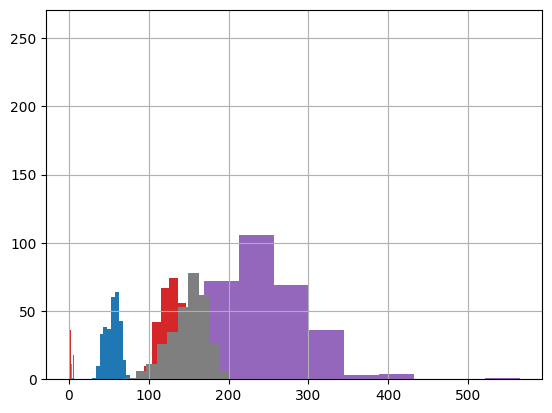
\includegraphics[keepaspectratio]{ans_files/figure-pdf/cell-4-output-2.png}}

The dataset contains missing values and have different scales and
distributions. For the variables, sex, fbs, exang are binary varialbes,
oldpeak is a continuous variable, and the remaining vriables are numeric
variables. There are 303 observations in the dataset.

\begin{enumerate}
\def\labelenumi{(\arabic{enumi})}
\setcounter{enumi}{3}
\tightlist
\item
\end{enumerate}

\begin{Shaded}
\begin{Highlighting}[]
\CommentTok{\# Convert the num column to a binary variable}
\NormalTok{scaled\_data[}\StringTok{\textquotesingle{}num\textquotesingle{}}\NormalTok{] }\OperatorTok{=}\NormalTok{ scaled\_data[}\StringTok{\textquotesingle{}num\textquotesingle{}}\NormalTok{].}\BuiltInTok{apply}\NormalTok{(}\KeywordTok{lambda}\NormalTok{ x: }\DecValTok{1} \ControlFlowTok{if}\NormalTok{ x }\OperatorTok{\textgreater{}} \DecValTok{0} \ControlFlowTok{else} \DecValTok{0}\NormalTok{)}
\end{Highlighting}
\end{Shaded}

\begin{enumerate}
\def\labelenumi{(\arabic{enumi})}
\setcounter{enumi}{4}
\tightlist
\item
\end{enumerate}

\begin{Shaded}
\begin{Highlighting}[]
\CommentTok{\# Correlation matrix}
\NormalTok{correlation\_matrix }\OperatorTok{=}\NormalTok{ scaled\_data.corr()}
\BuiltInTok{print}\NormalTok{(}\StringTok{"}\CharTok{\textbackslash{}n}\StringTok{Correlation matrix:"}\NormalTok{)}
\BuiltInTok{print}\NormalTok{(correlation\_matrix)}

\CommentTok{\# Visualize the correlation matrix}
\NormalTok{plt.figure(figsize}\OperatorTok{=}\NormalTok{(}\DecValTok{10}\NormalTok{, }\DecValTok{8}\NormalTok{))}
\NormalTok{sns.heatmap(correlation\_matrix, annot}\OperatorTok{=}\VariableTok{True}\NormalTok{, fmt}\OperatorTok{=}\StringTok{".2f"}\NormalTok{, cmap}\OperatorTok{=}\StringTok{\textquotesingle{}coolwarm\textquotesingle{}}\NormalTok{)}
\NormalTok{plt.title(}\StringTok{\textquotesingle{}Correlation Matrix\textquotesingle{}}\NormalTok{)}
\NormalTok{plt.show()}
\end{Highlighting}
\end{Shaded}

\begin{verbatim}

Correlation matrix:
               age       sex        cp  trestbps      chol       fbs  \
age       1.000000 -0.097542  0.104139  0.284946  0.208950  0.118530   
sex      -0.097542  1.000000  0.010084 -0.064456 -0.199915  0.047862   
cp        0.104139  0.010084  1.000000 -0.036077  0.072319 -0.039975   
trestbps  0.284946 -0.064456 -0.036077  1.000000  0.130120  0.175340   
chol      0.208950 -0.199915  0.072319  0.130120  1.000000  0.009841   
fbs       0.118530  0.047862 -0.039975  0.175340  0.009841  1.000000   
restecg   0.148868  0.021647  0.067505  0.146560  0.171043  0.069564   
thalach  -0.393806 -0.048663 -0.334422 -0.045351 -0.003432 -0.007854   
exang     0.091661  0.146201  0.384060  0.064762  0.061310  0.025665   
oldpeak   0.203805  0.102173  0.202277  0.189171  0.046564  0.005747   
slope     0.161770  0.037533  0.152050  0.117382 -0.004062  0.059894   
ca        0.362605  0.093185  0.233214  0.098773  0.119000  0.145478   
thal      0.127389  0.380936  0.265246  0.133554  0.014214  0.071358   
num       0.223120  0.276816  0.414446  0.150825  0.085164  0.025264   

           restecg   thalach     exang   oldpeak     slope        ca  \
age       0.148868 -0.393806  0.091661  0.203805  0.161770  0.362605   
sex       0.021647 -0.048663  0.146201  0.102173  0.037533  0.093185   
cp        0.067505 -0.334422  0.384060  0.202277  0.152050  0.233214   
trestbps  0.146560 -0.045351  0.064762  0.189171  0.117382  0.098773   
chol      0.171043 -0.003432  0.061310  0.046564 -0.004062  0.119000   
fbs       0.069564 -0.007854  0.025665  0.005747  0.059894  0.145478   
restecg   1.000000 -0.083389  0.084867  0.114133  0.133946  0.128343   
thalach  -0.083389  1.000000 -0.378103 -0.343085 -0.385601 -0.264246   
exang     0.084867 -0.378103  1.000000  0.288223  0.257748  0.145570   
oldpeak   0.114133 -0.343085  0.288223  1.000000  0.577537  0.295832   
slope     0.133946 -0.385601  0.257748  0.577537  1.000000  0.110119   
ca        0.128343 -0.264246  0.145570  0.295832  0.110119  1.000000   
thal      0.024531 -0.279631  0.329680  0.341004  0.287232  0.256382   
num       0.169202 -0.417167  0.431894  0.424510  0.339213  0.460442   

              thal       num  
age       0.127389  0.223120  
sex       0.380936  0.276816  
cp        0.265246  0.414446  
trestbps  0.133554  0.150825  
chol      0.014214  0.085164  
fbs       0.071358  0.025264  
restecg   0.024531  0.169202  
thalach  -0.279631 -0.417167  
exang     0.329680  0.431894  
oldpeak   0.341004  0.424510  
slope     0.287232  0.339213  
ca        0.256382  0.460442  
thal      1.000000  0.525689  
num       0.525689  1.000000  
\end{verbatim}

\pandocbounded{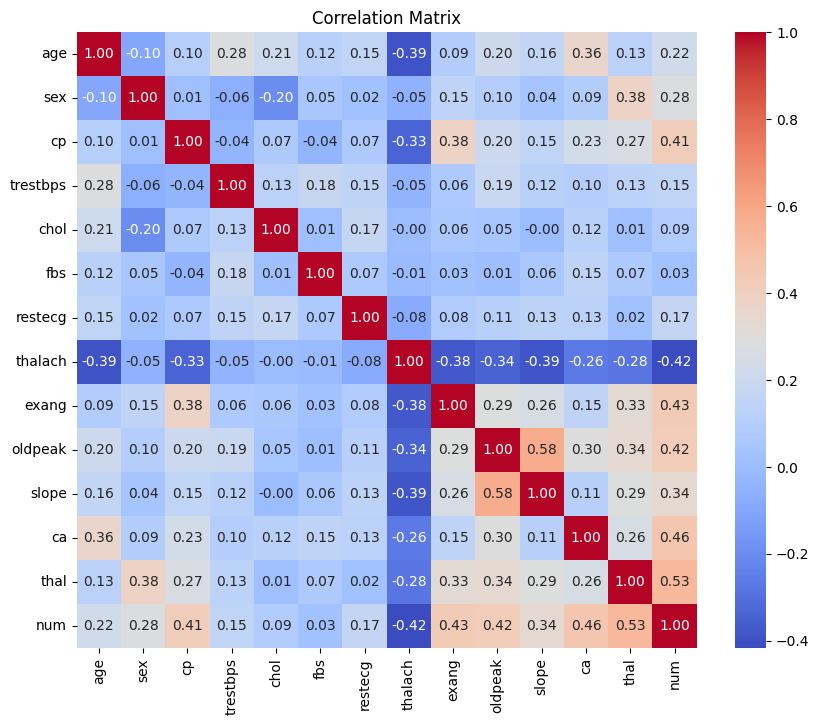
\includegraphics[keepaspectratio]{ans_files/figure-pdf/cell-6-output-2.png}}

From the correlation matrix, we can see that the features are not highly
correlated with each other. The top-3 variable with highest correlation
with num is thal, ca, and exang.

\begin{enumerate}
\def\labelenumi{(\arabic{enumi})}
\setcounter{enumi}{5}
\tightlist
\item
\end{enumerate}

\begin{Shaded}
\begin{Highlighting}[]
\NormalTok{scaled\_data.dropna(inplace}\OperatorTok{=}\VariableTok{True}\NormalTok{)}
\NormalTok{num\_observations\_after\_drop }\OperatorTok{=}\NormalTok{ scaled\_data.shape[}\DecValTok{0}\NormalTok{]}

\BuiltInTok{print}\NormalTok{(num\_observations\_after\_drop)}
\end{Highlighting}
\end{Shaded}

\begin{verbatim}
297
\end{verbatim}

There are 297 observations after dropping the missing values.

\begin{enumerate}
\def\labelenumi{(\arabic{enumi})}
\setcounter{enumi}{6}
\tightlist
\item
\end{enumerate}

\begin{Shaded}
\begin{Highlighting}[]

\NormalTok{categorical\_cols }\OperatorTok{=}\NormalTok{ [}\StringTok{\textquotesingle{}sex\textquotesingle{}}\NormalTok{, }\StringTok{\textquotesingle{}cp\textquotesingle{}}\NormalTok{, }\StringTok{\textquotesingle{}fbs\textquotesingle{}}\NormalTok{, }\StringTok{\textquotesingle{}restecg\textquotesingle{}}\NormalTok{, }\StringTok{\textquotesingle{}exang\textquotesingle{}}\NormalTok{, }\StringTok{\textquotesingle{}slope\textquotesingle{}}\NormalTok{, }\StringTok{\textquotesingle{}ca\textquotesingle{}}\NormalTok{, }\StringTok{\textquotesingle{}thal\textquotesingle{}}\NormalTok{, }\StringTok{\textquotesingle{}num\textquotesingle{}}\NormalTok{]}
\NormalTok{X\_cluster }\OperatorTok{=}\NormalTok{ scaled\_data.drop(columns }\OperatorTok{=}\NormalTok{ categorical\_cols)}

\NormalTok{scaler }\OperatorTok{=}\NormalTok{ StandardScaler()}
\NormalTok{X\_scaled }\OperatorTok{=}\NormalTok{ scaler.fit\_transform(X\_cluster)}


\NormalTok{kmeans }\OperatorTok{=}\NormalTok{ KMeans(n\_clusters }\OperatorTok{=} \DecValTok{3}\NormalTok{, random\_state }\OperatorTok{=} \DecValTok{1}\NormalTok{) }\CommentTok{\#choose the number of clusters = 3 due to previous knowledge}
\NormalTok{clusters }\OperatorTok{=}\NormalTok{ kmeans.fit\_predict(X\_scaled)}

\NormalTok{pca }\OperatorTok{=}\NormalTok{ PCA(n\_components }\OperatorTok{=} \DecValTok{2}\NormalTok{)}
\NormalTok{X\_pca }\OperatorTok{=}\NormalTok{ pca.fit\_transform(X\_scaled)}

\NormalTok{plt.figure(figsize }\OperatorTok{=}\NormalTok{ (}\DecValTok{8}\NormalTok{,}\DecValTok{6}\NormalTok{))}
\NormalTok{sns.scatterplot(x }\OperatorTok{=}\NormalTok{ X\_pca[:, }\DecValTok{0}\NormalTok{], y }\OperatorTok{=}\NormalTok{ X\_pca[:, }\DecValTok{1}\NormalTok{], hue }\OperatorTok{=}\NormalTok{ clusters, palette }\OperatorTok{=} \StringTok{\textquotesingle{}Set2\textquotesingle{}}\NormalTok{ , s }\OperatorTok{=} \DecValTok{40}\NormalTok{)}

\NormalTok{plt.title(}\StringTok{\textquotesingle{}KMeans Clustering (after PCA projection)\textquotesingle{}}\NormalTok{)}
\NormalTok{plt.show()}
\end{Highlighting}
\end{Shaded}

\pandocbounded{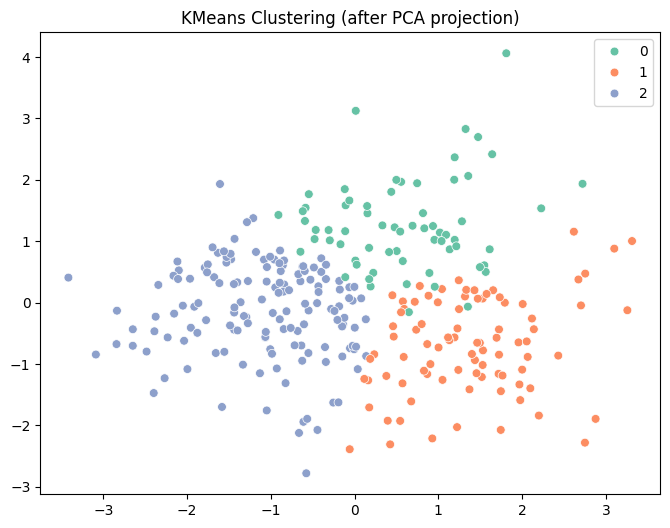
\includegraphics[keepaspectratio]{ans_files/figure-pdf/cell-8-output-1.png}}

\begin{enumerate}
\def\labelenumi{(\arabic{enumi})}
\setcounter{enumi}{7}
\tightlist
\item
\end{enumerate}

\begin{Shaded}
\begin{Highlighting}[]
\NormalTok{X }\OperatorTok{=}\NormalTok{ scaled\_data.drop(columns}\OperatorTok{=}\NormalTok{[}\StringTok{"num"}\NormalTok{])}
\NormalTok{y }\OperatorTok{=}\NormalTok{ scaled\_data[}\StringTok{"num"}\NormalTok{]}

\NormalTok{X\_train, X\_test, y\_train, y\_test }\OperatorTok{=}\NormalTok{ train\_test\_split(}
\NormalTok{    X, y, test\_size}\OperatorTok{=}\FloatTok{0.3}\NormalTok{, random\_state}\OperatorTok{=}\DecValTok{1}\NormalTok{, stratify}\OperatorTok{=}\NormalTok{y}
\NormalTok{)}

\BuiltInTok{print}\NormalTok{(}\SpecialStringTok{f"Training set size: }\SpecialCharTok{\{}\NormalTok{X\_train}\SpecialCharTok{.}\NormalTok{shape[}\DecValTok{0}\NormalTok{]}\SpecialCharTok{\}}\SpecialStringTok{"}\NormalTok{)}
\BuiltInTok{print}\NormalTok{(}\SpecialStringTok{f"Testing set size: }\SpecialCharTok{\{}\NormalTok{X\_test}\SpecialCharTok{.}\NormalTok{shape[}\DecValTok{0}\NormalTok{]}\SpecialCharTok{\}}\SpecialStringTok{"}\NormalTok{)}
\end{Highlighting}
\end{Shaded}

\begin{verbatim}
Training set size: 207
Testing set size: 90
\end{verbatim}

\begin{enumerate}
\def\labelenumi{(\arabic{enumi})}
\setcounter{enumi}{8}
\tightlist
\item
\end{enumerate}

We select:

\begin{enumerate}
\def\labelenumi{\arabic{enumi}.}
\tightlist
\item
  Logistic Regression
\end{enumerate}

Logistic regression always used for binary classification problems.
Because it is really efficiency for small/medium datasets. The structure
of it is easy and has great interpretability. In this case we are
analysising the heart disease dataset, and by previous knowledge we know
logistic regression is suitale for this kind of dataset. So the first
one we choose is logistic regression.

\begin{enumerate}
\def\labelenumi{\arabic{enumi}.}
\setcounter{enumi}{1}
\tightlist
\item
  Decision Tree
\end{enumerate}

Decision tree is a very well understood model that divides data into
different categories step by step by constantly making ``yes'' and
``no'' judgments on features. It is very easy to operate because we
don't need to standardize the data in advance, and it can handle
different types of data at the same time. I think its biggest advantage
is that it has a clear structure, and it can draw very graphical
diagrams to see how to make decisions at each step, which is very
helpful for medical data analysis, because the model is very explanatory
and easy to understand. For example, let's judge each item in this data
on a finger-by-finger basis.

\begin{enumerate}
\def\labelenumi{(\arabic{enumi})}
\setcounter{enumi}{9}
\tightlist
\item
\end{enumerate}

We choose accuracy and precision.

\begin{enumerate}
\def\labelenumi{\arabic{enumi}.}
\tightlist
\item
  Accuracy:
\end{enumerate}

formula when calculating `Accuracy = (TP + TN) / (TP + TN + FP + FN)' TP
is True Positive, TN is True Negative; FP is False Positive, FN is False
Negative.

It is one of the most commonly used metrics to measure the overall
performance of a classification model. It shows how many times the model
predicted correctly and what percentage of the total predictions were
made.

\begin{enumerate}
\def\labelenumi{\arabic{enumi}.}
\setcounter{enumi}{1}
\tightlist
\item
  Sensitivity:
\end{enumerate}

Formula when calculating `Sensitivity = TP / (TP + FN)'\\
TP is True Positive, FN is False Negative.

Sensitivity measures how well the model identifies actual positive
cases. In other words, sensitivity shows what proportion of people who
are actually ``have problem'' were correctly predicted as ``have
problem/sick'' by the model. A high sensitivity means the model is good
at detecting all real cases, even sometimes it maybe too sensitive. But
if we cannot identify someone is actual ``have problem'' it may lead to
very bad situation.

\begin{enumerate}
\def\labelenumi{(\arabic{enumi})}
\setcounter{enumi}{10}
\tightlist
\item
\end{enumerate}

\begin{Shaded}
\begin{Highlighting}[]
\CommentTok{\# identify optimal tuning parameters using cross validation}
\NormalTok{depth\_range }\OperatorTok{=} \BuiltInTok{range}\NormalTok{(}\DecValTok{1}\NormalTok{, }\DecValTok{20}\NormalTok{)}
\NormalTok{cv\_scores }\OperatorTok{=}\NormalTok{ []}
\ControlFlowTok{for}\NormalTok{ k }\KeywordTok{in}\NormalTok{ depth\_range:}
\NormalTok{    heart\_disease\_log }\OperatorTok{=}\NormalTok{ LogisticRegression(max\_iter}\OperatorTok{=}\DecValTok{120}\NormalTok{, C}\OperatorTok{=}\NormalTok{k)}
\CommentTok{\# 5{-}fold cross{-}validation using accuracy}
\NormalTok{    cv\_scores\_k }\OperatorTok{=}\NormalTok{ cross\_val\_score(}
\NormalTok{        heart\_disease\_log,}
\NormalTok{        X\_train,}
\NormalTok{        y\_train,}
\NormalTok{        cv}\OperatorTok{=}\DecValTok{5}\NormalTok{,}
\NormalTok{        scoring}\OperatorTok{=}\StringTok{\textquotesingle{}accuracy\textquotesingle{}}
\NormalTok{    )}
\CommentTok{\# append the average accuracy across all folds}
\NormalTok{    cv\_scores.append(np.mean(cv\_scores\_k))}
\NormalTok{plt.plot(depth\_range, cv\_scores)}
\NormalTok{plt.xlabel(}\StringTok{\textquotesingle{}depth\textquotesingle{}}\NormalTok{)}
\NormalTok{plt.ylabel(}\StringTok{\textquotesingle{}CV accuracy\textquotesingle{}}\NormalTok{)}
\NormalTok{plt.xticks(}\BuiltInTok{range}\NormalTok{(}\DecValTok{1}\NormalTok{,}\DecValTok{20}\NormalTok{))}
\NormalTok{plt.show()}

\NormalTok{optimal\_depth\_index }\OperatorTok{=}\NormalTok{ np.argmax(cv\_scores)}
\NormalTok{optimal\_depth }\OperatorTok{=}\NormalTok{ depth\_range[optimal\_depth\_index]}

\BuiltInTok{print}\NormalTok{(}\StringTok{"Optimal max\_depth: "}\NormalTok{, optimal\_depth)}

\CommentTok{\# train logistic regression model }
\NormalTok{heart\_disease\_log }\OperatorTok{=}\NormalTok{ LogisticRegression(max\_iter}\OperatorTok{=}\DecValTok{120}\NormalTok{, C}\OperatorTok{=}\NormalTok{optimal\_depth)}
\NormalTok{heart\_disease\_log.fit(X\_train, y\_train)}
\end{Highlighting}
\end{Shaded}

\pandocbounded{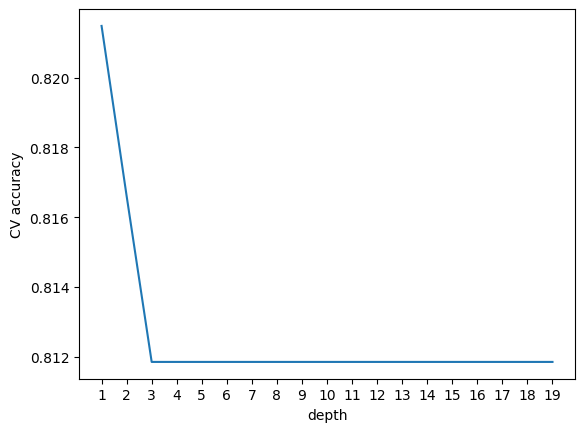
\includegraphics[keepaspectratio]{ans_files/figure-pdf/cell-10-output-1.png}}

\begin{verbatim}
Optimal max_depth:  1
\end{verbatim}

\begin{verbatim}
LogisticRegression(C=1, max_iter=120)
\end{verbatim}

The optimal tuning parameter for logistic regression is max depth k: 1.

\begin{Shaded}
\begin{Highlighting}[]
\CommentTok{\# identify optimal tuning parameters using cross validation}
\NormalTok{depth\_range }\OperatorTok{=} \BuiltInTok{range}\NormalTok{(}\DecValTok{1}\NormalTok{, }\DecValTok{20}\NormalTok{)}
\NormalTok{cv\_scores }\OperatorTok{=}\NormalTok{ []}
\ControlFlowTok{for}\NormalTok{ k }\KeywordTok{in}\NormalTok{ depth\_range:}
\NormalTok{    dt }\OperatorTok{=}\NormalTok{ DecisionTreeClassifier(}
\NormalTok{    criterion}\OperatorTok{=}\StringTok{\textquotesingle{}gini\textquotesingle{}}\NormalTok{, }
\NormalTok{    random\_state}\OperatorTok{=}\DecValTok{0}\NormalTok{,}
\NormalTok{    max\_depth}\OperatorTok{=}\NormalTok{k}
\NormalTok{    )}

\NormalTok{    cv\_scores\_k }\OperatorTok{=}\NormalTok{ cross\_val\_score(}
\NormalTok{        dt,}
\NormalTok{        X\_train,}
\NormalTok{        y\_train,}
\NormalTok{        cv}\OperatorTok{=}\DecValTok{5}\NormalTok{,}
\NormalTok{        scoring}\OperatorTok{=}\StringTok{\textquotesingle{}accuracy\textquotesingle{}}
\NormalTok{    )}
\NormalTok{    cv\_scores.append(np.mean(cv\_scores\_k))}
\NormalTok{plt.plot(depth\_range, cv\_scores)}
\NormalTok{plt.xlabel(}\StringTok{\textquotesingle{}depth\textquotesingle{}}\NormalTok{)}
\NormalTok{plt.ylabel(}\StringTok{\textquotesingle{}CV accuracy\textquotesingle{}}\NormalTok{)}
\NormalTok{plt.xticks(}\BuiltInTok{range}\NormalTok{(}\DecValTok{1}\NormalTok{,}\DecValTok{20}\NormalTok{))}
\NormalTok{plt.show()}

\NormalTok{optimal\_depth\_index }\OperatorTok{=}\NormalTok{ np.argmax(cv\_scores)}
\NormalTok{optimal\_depth }\OperatorTok{=}\NormalTok{ depth\_range[optimal\_depth\_index]}

\BuiltInTok{print}\NormalTok{(}\StringTok{"Optimal max\_depth: "}\NormalTok{, optimal\_depth)}

\CommentTok{\# train decision tree model}
\NormalTok{heart\_disease\_dt }\OperatorTok{=}\NormalTok{ DecisionTreeClassifier(}
\NormalTok{    criterion}\OperatorTok{=}\StringTok{\textquotesingle{}gini\textquotesingle{}}\NormalTok{,}
\NormalTok{    random\_state}\OperatorTok{=}\DecValTok{0}\NormalTok{,}
\NormalTok{    max\_depth}\OperatorTok{=}\DecValTok{3}
\NormalTok{)}
\NormalTok{heart\_disease\_dt.fit(X\_train, y\_train)}
\end{Highlighting}
\end{Shaded}

\pandocbounded{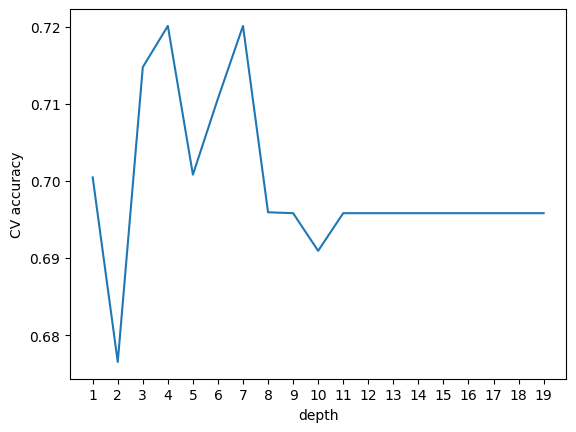
\includegraphics[keepaspectratio]{ans_files/figure-pdf/cell-11-output-1.png}}

\begin{verbatim}
Optimal max_depth:  7
\end{verbatim}

\begin{verbatim}
DecisionTreeClassifier(max_depth=3, random_state=0)
\end{verbatim}

The optimal tuning parameter for decision tree is optimal max depth: 7.

\begin{enumerate}
\def\labelenumi{(\arabic{enumi})}
\setcounter{enumi}{11}
\tightlist
\item
\end{enumerate}

\begin{Shaded}
\begin{Highlighting}[]
\CommentTok{\# Apply Step{-}wise subset selection to descision tree}
\NormalTok{sfs }\OperatorTok{=}\NormalTok{ SFS(}
\NormalTok{    estimator}\OperatorTok{=}\NormalTok{heart\_disease\_dt,}
\NormalTok{    k\_features}\OperatorTok{=}\NormalTok{(}\DecValTok{1}\NormalTok{, }\DecValTok{8}\NormalTok{),}
\NormalTok{    forward}\OperatorTok{=}\VariableTok{True}\NormalTok{,}
\NormalTok{    floating}\OperatorTok{=}\VariableTok{False}\NormalTok{,}
\NormalTok{    scoring}\OperatorTok{=}\StringTok{\textquotesingle{}accuracy\textquotesingle{}}\NormalTok{,  }
\NormalTok{    cv}\OperatorTok{=}\DecValTok{5}\NormalTok{,}
\NormalTok{)}
\NormalTok{sfs.fit(X\_train, y\_train)}

\CommentTok{\# identify optimal tuning parameters}
\NormalTok{selected\_features }\OperatorTok{=}\NormalTok{ X\_train.columns[}\BuiltInTok{list}\NormalTok{(sfs.k\_feature\_idx\_)]}
\NormalTok{X\_train\_sfs }\OperatorTok{=}\NormalTok{ X\_train[selected\_features]}
\NormalTok{X\_test\_sfs }\OperatorTok{=}\NormalTok{ X\_test[selected\_features]}

\NormalTok{depth\_range }\OperatorTok{=} \BuiltInTok{range}\NormalTok{(}\DecValTok{1}\NormalTok{, }\DecValTok{20}\NormalTok{)}
\NormalTok{cv\_scores }\OperatorTok{=}\NormalTok{ []}
\ControlFlowTok{for}\NormalTok{ k }\KeywordTok{in}\NormalTok{ depth\_range:}
\NormalTok{    dt }\OperatorTok{=}\NormalTok{ DecisionTreeClassifier(}
\NormalTok{    criterion}\OperatorTok{=}\StringTok{\textquotesingle{}gini\textquotesingle{}}\NormalTok{, }
\NormalTok{    random\_state}\OperatorTok{=}\DecValTok{0}\NormalTok{,}
\NormalTok{    max\_depth}\OperatorTok{=}\NormalTok{k}
\NormalTok{    )}

\NormalTok{    cv\_scores\_k }\OperatorTok{=}\NormalTok{ cross\_val\_score(}
\NormalTok{        dt,}
\NormalTok{        X\_train\_sfs,}
\NormalTok{        y\_train,}
\NormalTok{        cv}\OperatorTok{=}\DecValTok{5}\NormalTok{,}
\NormalTok{        scoring}\OperatorTok{=}\StringTok{\textquotesingle{}accuracy\textquotesingle{}}
\NormalTok{    )}
\NormalTok{    cv\_scores.append(np.mean(cv\_scores\_k))}

\NormalTok{optimal\_depth\_index }\OperatorTok{=}\NormalTok{ np.argmax(cv\_scores)}
\NormalTok{optimal\_depth }\OperatorTok{=}\NormalTok{ depth\_range[optimal\_depth\_index]}

\BuiltInTok{print}\NormalTok{(}\StringTok{"Optimal max\_depth: "}\NormalTok{, optimal\_depth)}

\CommentTok{\# train decision tree model with selected features}
\NormalTok{m\_sfs }\OperatorTok{=}\NormalTok{ DecisionTreeClassifier(}
\NormalTok{    criterion}\OperatorTok{=}\StringTok{\textquotesingle{}gini\textquotesingle{}}\NormalTok{,}
\NormalTok{    random\_state}\OperatorTok{=}\DecValTok{0}\NormalTok{,}
\NormalTok{    max\_depth}\OperatorTok{=}\NormalTok{optimal\_depth}
\NormalTok{)}
\NormalTok{m\_sfs.fit(X\_train\_sfs, y\_train)}
\end{Highlighting}
\end{Shaded}

\begin{verbatim}
Optimal max_depth:  3
\end{verbatim}

\begin{verbatim}
DecisionTreeClassifier(max_depth=3, random_state=0)
\end{verbatim}

The optimal tuning parameter for decision tree is optimal max depth: 3.

\begin{enumerate}
\def\labelenumi{(\arabic{enumi})}
\setcounter{enumi}{12}
\tightlist
\item
\end{enumerate}

\begin{Shaded}
\begin{Highlighting}[]
\CommentTok{\# confusion matrix for logistic regression}
\NormalTok{y\_test\_hat }\OperatorTok{=}\NormalTok{ heart\_disease\_log.predict(X\_test)}
\NormalTok{cm\_log }\OperatorTok{=}\NormalTok{ confusion\_matrix(y\_test, y\_test\_hat)}
\NormalTok{total1 }\OperatorTok{=} \BuiltInTok{sum}\NormalTok{(}\BuiltInTok{sum}\NormalTok{(cm\_log))}
\NormalTok{accuracy\_log }\OperatorTok{=}\NormalTok{ (cm\_log[}\DecValTok{0}\NormalTok{,}\DecValTok{0}\NormalTok{]}\OperatorTok{+}\NormalTok{cm\_log[}\DecValTok{1}\NormalTok{,}\DecValTok{1}\NormalTok{])}\OperatorTok{/}\NormalTok{total1}
\BuiltInTok{print}\NormalTok{(}\StringTok{"Logistic Regression Accuracy: "}\NormalTok{, accuracy\_log)}
\NormalTok{sensitivity\_log }\OperatorTok{=}\NormalTok{ cm\_log[}\DecValTok{1}\NormalTok{,}\DecValTok{1}\NormalTok{]}\OperatorTok{/}\NormalTok{(cm\_log[}\DecValTok{1}\NormalTok{,}\DecValTok{0}\NormalTok{]}\OperatorTok{+}\NormalTok{cm\_log[}\DecValTok{1}\NormalTok{,}\DecValTok{1}\NormalTok{]) }
\BuiltInTok{print}\NormalTok{(}\StringTok{"Logistic Regression Sensitivity: "}\NormalTok{, sensitivity\_log)}

\NormalTok{y\_pred\_dt }\OperatorTok{=}\NormalTok{ heart\_disease\_dt.predict(X\_test)}
\CommentTok{\# confusion matrix for decision tree}
\NormalTok{cm\_dt }\OperatorTok{=}\NormalTok{ confusion\_matrix(y\_test, y\_pred\_dt)}
\NormalTok{total2 }\OperatorTok{=} \BuiltInTok{sum}\NormalTok{(}\BuiltInTok{sum}\NormalTok{(cm\_dt))}
\NormalTok{accuracy\_dt }\OperatorTok{=}\NormalTok{ (cm\_dt[}\DecValTok{0}\NormalTok{,}\DecValTok{0}\NormalTok{]}\OperatorTok{+}\NormalTok{cm\_dt[}\DecValTok{1}\NormalTok{,}\DecValTok{1}\NormalTok{])}\OperatorTok{/}\NormalTok{total2}
\BuiltInTok{print}\NormalTok{(}\StringTok{"Decision Tree Accuracy: "}\NormalTok{, accuracy\_dt)}
\NormalTok{sensitivity\_dt }\OperatorTok{=}\NormalTok{ cm\_dt[}\DecValTok{1}\NormalTok{,}\DecValTok{1}\NormalTok{]}\OperatorTok{/}\NormalTok{(cm\_dt[}\DecValTok{1}\NormalTok{,}\DecValTok{0}\NormalTok{]}\OperatorTok{+}\NormalTok{cm\_dt[}\DecValTok{1}\NormalTok{,}\DecValTok{1}\NormalTok{])}
\BuiltInTok{print}\NormalTok{(}\StringTok{"Decision Tree Sensitivity: "}\NormalTok{, sensitivity\_dt)}

\NormalTok{y\_pred\_sfs }\OperatorTok{=}\NormalTok{ m\_sfs.predict(X\_test\_sfs)}
\CommentTok{\# confusion matrix for decision tree with selected features}
\NormalTok{cm\_sfs }\OperatorTok{=}\NormalTok{ confusion\_matrix(y\_test, y\_pred\_sfs)}
\NormalTok{total3 }\OperatorTok{=} \BuiltInTok{sum}\NormalTok{(}\BuiltInTok{sum}\NormalTok{(cm\_sfs))}
\NormalTok{accuracy\_sfs }\OperatorTok{=}\NormalTok{ (cm\_sfs[}\DecValTok{0}\NormalTok{,}\DecValTok{0}\NormalTok{]}\OperatorTok{+}\NormalTok{cm\_sfs[}\DecValTok{1}\NormalTok{,}\DecValTok{1}\NormalTok{])}\OperatorTok{/}\NormalTok{total3}
\BuiltInTok{print}\NormalTok{(}\StringTok{"Decision Tree with Selected Features Accuracy: "}\NormalTok{, accuracy\_sfs)}
\NormalTok{sensitivity\_sfs }\OperatorTok{=}\NormalTok{ cm\_sfs[}\DecValTok{1}\NormalTok{,}\DecValTok{1}\NormalTok{]}\OperatorTok{/}\NormalTok{(cm\_sfs[}\DecValTok{1}\NormalTok{,}\DecValTok{0}\NormalTok{]}\OperatorTok{+}\NormalTok{cm\_sfs[}\DecValTok{1}\NormalTok{,}\DecValTok{1}\NormalTok{])}
\BuiltInTok{print}\NormalTok{(}\StringTok{"Decision Tree with Selected Features Sensitivity: "}\NormalTok{, sensitivity\_sfs)}
\end{Highlighting}
\end{Shaded}

\begin{verbatim}
Logistic Regression Accuracy:  0.8444444444444444
Logistic Regression Sensitivity:  0.7619047619047619
Decision Tree Accuracy:  0.7444444444444445
Decision Tree Sensitivity:  0.7857142857142857
Decision Tree with Selected Features Accuracy:  0.7555555555555555
Decision Tree with Selected Features Sensitivity:  0.8095238095238095
\end{verbatim}

The Logistic Regression model has a higher accuracy than the Decision
Tree model. However, the Decision Tree model has a higher sensitivity,
which means it is better at identifying positive cases.\\
Both accuracy and sensitivity for Decision Tree model with SFS are bit
higher than the original Decision Tree model. This indicates that
feature selection has improved the performance of the classifier.

\begin{enumerate}
\def\labelenumi{(\arabic{enumi})}
\setcounter{enumi}{13}
\tightlist
\item
\end{enumerate}

\begin{Shaded}
\begin{Highlighting}[]
\CommentTok{\# The best interpretable model identified in (13) is logistic regression.}
\NormalTok{coefficients }\OperatorTok{=}\NormalTok{ heart\_disease\_log.coef\_[}\DecValTok{0}\NormalTok{]}
\NormalTok{feature\_importance }\OperatorTok{=}\NormalTok{ pd.DataFrame(}
\NormalTok{    \{}\StringTok{\textquotesingle{}Feature\textquotesingle{}}\NormalTok{: X\_train.columns,}
     \StringTok{\textquotesingle{}Coefficient\textquotesingle{}}\NormalTok{: coefficients\}}
\NormalTok{)}
\NormalTok{feature\_importance[}\StringTok{\textquotesingle{}Importance\textquotesingle{}}\NormalTok{] }\OperatorTok{=}\NormalTok{ np.}\BuiltInTok{abs}\NormalTok{(feature\_importance[}\StringTok{\textquotesingle{}Coefficient\textquotesingle{}}\NormalTok{])}
\NormalTok{feature\_importance }\OperatorTok{=}\NormalTok{ feature\_importance.sort\_values(by}\OperatorTok{=}\StringTok{\textquotesingle{}Importance\textquotesingle{}}\NormalTok{, ascending}\OperatorTok{=}\VariableTok{False}\NormalTok{)}
\NormalTok{plt.figure(figsize}\OperatorTok{=}\NormalTok{(}\DecValTok{10}\NormalTok{, }\DecValTok{6}\NormalTok{))}
\NormalTok{sns.barplot(x}\OperatorTok{=}\StringTok{\textquotesingle{}Importance\textquotesingle{}}\NormalTok{, y}\OperatorTok{=}\StringTok{\textquotesingle{}Feature\textquotesingle{}}\NormalTok{, data}\OperatorTok{=}\NormalTok{feature\_importance, palette}\OperatorTok{=}\StringTok{\textquotesingle{}viridis\textquotesingle{}}\NormalTok{)}
\NormalTok{plt.title(}\StringTok{\textquotesingle{}Feature Importance from Logistic Regression\textquotesingle{}}\NormalTok{)}
\NormalTok{plt.xlabel(}\StringTok{\textquotesingle{}Absolute Coefficient Value\textquotesingle{}}\NormalTok{)}
\NormalTok{plt.ylabel(}\StringTok{\textquotesingle{}Feature\textquotesingle{}}\NormalTok{)}
\NormalTok{plt.show()}
\end{Highlighting}
\end{Shaded}

\begin{verbatim}
/tmp/ipykernel_693798/1559183592.py:10: FutureWarning: 

Passing `palette` without assigning `hue` is deprecated and will be removed in v0.14.0. Assign the `y` variable to `hue` and set `legend=False` for the same effect.

  sns.barplot(x='Importance', y='Feature', data=feature_importance, palette='viridis')
\end{verbatim}

\pandocbounded{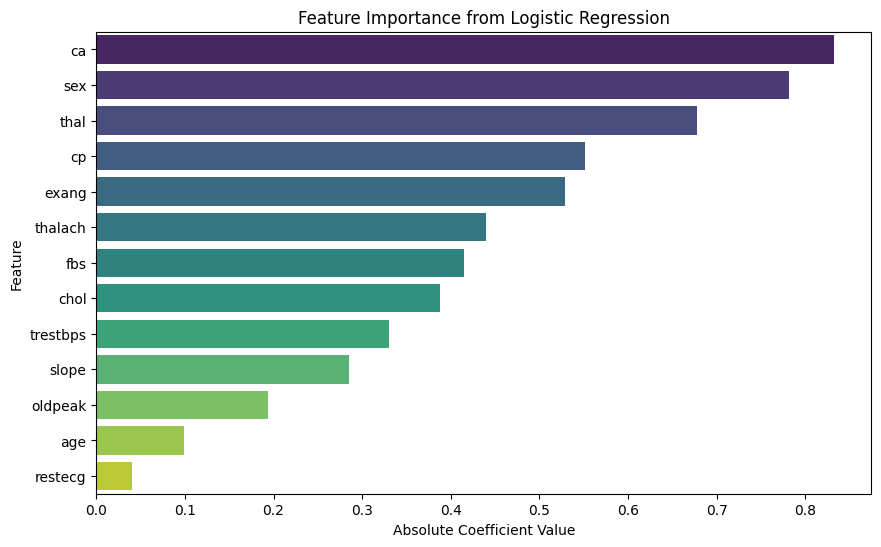
\includegraphics[keepaspectratio]{ans_files/figure-pdf/cell-14-output-2.png}}

The most important predictor variables is `ca', which is the number of
major vessels (0-3) colored by fluoroscopy. This variable has a positive
coefficient, indicating that as the number of major vessels increases,
the likelihood of having heart disease also increases. This suggests
that individuals with more major vessels are at a higher risk of heart
disease.

\begin{enumerate}
\def\labelenumi{(\arabic{enumi})}
\setcounter{enumi}{14}
\tightlist
\item
\end{enumerate}

\begin{Shaded}
\begin{Highlighting}[]
\CommentTok{\# Using Random Forest Classifier}
\CommentTok{\# Define the parameter grid}
\NormalTok{param\_grid }\OperatorTok{=}\NormalTok{ \{}
    \StringTok{\textquotesingle{}n\_estimators\textquotesingle{}}\NormalTok{: [}\DecValTok{100}\NormalTok{, }\DecValTok{200}\NormalTok{, }\DecValTok{300}\NormalTok{],}
    \StringTok{\textquotesingle{}max\_depth\textquotesingle{}}\NormalTok{: [}\VariableTok{None}\NormalTok{, }\DecValTok{10}\NormalTok{, }\DecValTok{20}\NormalTok{, }\DecValTok{30}\NormalTok{],}
    \StringTok{\textquotesingle{}min\_samples\_split\textquotesingle{}}\NormalTok{: [}\DecValTok{2}\NormalTok{, }\DecValTok{5}\NormalTok{, }\DecValTok{10}\NormalTok{],}
    \StringTok{\textquotesingle{}min\_samples\_leaf\textquotesingle{}}\NormalTok{: [}\DecValTok{1}\NormalTok{, }\DecValTok{2}\NormalTok{, }\DecValTok{4}\NormalTok{]}
\NormalTok{\}}

\CommentTok{\# Create a Random Forest Classifier}
\NormalTok{rf }\OperatorTok{=}\NormalTok{ RandomForestClassifier(random\_state}\OperatorTok{=}\DecValTok{42}\NormalTok{)}

\CommentTok{\# Perform Grid Search with Cross{-}Validation}
\NormalTok{grid\_search }\OperatorTok{=}\NormalTok{ GridSearchCV(estimator}\OperatorTok{=}\NormalTok{rf, param\_grid}\OperatorTok{=}\NormalTok{param\_grid,}
\NormalTok{                           scoring}\OperatorTok{=}\StringTok{\textquotesingle{}accuracy\textquotesingle{}}\NormalTok{, cv}\OperatorTok{=}\DecValTok{5}\NormalTok{, verbose}\OperatorTok{=}\DecValTok{2}\NormalTok{, n\_jobs}\OperatorTok{={-}}\DecValTok{1}\NormalTok{)}

\CommentTok{\# Fit the model}
\NormalTok{grid\_search.fit(X\_train, y\_train)}

\CommentTok{\# Get the best parameters}
\NormalTok{best\_params }\OperatorTok{=}\NormalTok{ grid\_search.best\_params\_}
\BuiltInTok{print}\NormalTok{(}\StringTok{"Best parameters for Random Forest Classifier:"}\NormalTok{)}
\BuiltInTok{print}\NormalTok{(best\_params)}

\CommentTok{\# Train the Random Forest Classifier with the best parameters}
\NormalTok{rf\_best }\OperatorTok{=}\NormalTok{ RandomForestClassifier(}\OperatorTok{**}\NormalTok{best\_params, random\_state}\OperatorTok{=}\DecValTok{42}\NormalTok{)}
\NormalTok{rf\_best.fit(X\_train, y\_train)}

\CommentTok{\# Make predictions}
\NormalTok{y\_pred\_rf }\OperatorTok{=}\NormalTok{ rf\_best.predict(X\_test)}

\CommentTok{\# Confusion matrix for Random Forest Classifier}
\NormalTok{cm\_rf }\OperatorTok{=}\NormalTok{ confusion\_matrix(y\_test, y\_pred\_rf)}
\NormalTok{total4 }\OperatorTok{=} \BuiltInTok{sum}\NormalTok{(}\BuiltInTok{sum}\NormalTok{(cm\_rf))}
\NormalTok{accuracy\_rf }\OperatorTok{=}\NormalTok{ (cm\_rf[}\DecValTok{0}\NormalTok{,}\DecValTok{0}\NormalTok{]}\OperatorTok{+}\NormalTok{cm\_rf[}\DecValTok{1}\NormalTok{,}\DecValTok{1}\NormalTok{])}\OperatorTok{/}\NormalTok{total4}
\BuiltInTok{print}\NormalTok{(}\StringTok{"Random Forest Classifier Accuracy: "}\NormalTok{, accuracy\_rf)}
\NormalTok{sensitivity\_rf }\OperatorTok{=}\NormalTok{ cm\_rf[}\DecValTok{1}\NormalTok{,}\DecValTok{1}\NormalTok{]}\OperatorTok{/}\NormalTok{(cm\_rf[}\DecValTok{1}\NormalTok{,}\DecValTok{0}\NormalTok{]}\OperatorTok{+}\NormalTok{cm\_rf[}\DecValTok{1}\NormalTok{,}\DecValTok{1}\NormalTok{])}
\BuiltInTok{print}\NormalTok{(}\StringTok{"Random Forest Classifier Sensitivity: "}\NormalTok{, sensitivity\_rf)}

\CommentTok{\# Feature importance from Random Forest Classifier}
\NormalTok{feature\_importance\_rf }\OperatorTok{=}\NormalTok{ pd.DataFrame(}
\NormalTok{    \{}\StringTok{\textquotesingle{}Feature\textquotesingle{}}\NormalTok{: X\_train.columns,}
     \StringTok{\textquotesingle{}Importance\textquotesingle{}}\NormalTok{: rf\_best.feature\_importances\_\}}
\NormalTok{)}
\NormalTok{feature\_importance\_rf }\OperatorTok{=}\NormalTok{ feature\_importance\_rf.sort\_values(by}\OperatorTok{=}\StringTok{\textquotesingle{}Importance\textquotesingle{}}\NormalTok{, ascending}\OperatorTok{=}\VariableTok{False}\NormalTok{)}
\NormalTok{plt.figure(figsize}\OperatorTok{=}\NormalTok{(}\DecValTok{10}\NormalTok{, }\DecValTok{6}\NormalTok{))}
\NormalTok{sns.barplot(x}\OperatorTok{=}\StringTok{\textquotesingle{}Importance\textquotesingle{}}\NormalTok{, y}\OperatorTok{=}\StringTok{\textquotesingle{}Feature\textquotesingle{}}\NormalTok{, data}\OperatorTok{=}\NormalTok{feature\_importance\_rf, palette}\OperatorTok{=}\StringTok{\textquotesingle{}viridis\textquotesingle{}}\NormalTok{)}
\NormalTok{plt.title(}\StringTok{\textquotesingle{}Feature Importance from Random Forest Classifier\textquotesingle{}}\NormalTok{)}
\NormalTok{plt.xlabel(}\StringTok{\textquotesingle{}Importance\textquotesingle{}}\NormalTok{)}
\NormalTok{plt.ylabel(}\StringTok{\textquotesingle{}Feature\textquotesingle{}}\NormalTok{)}
\end{Highlighting}
\end{Shaded}

\begin{verbatim}
Fitting 5 folds for each of 108 candidates, totalling 540 fits
[CV] END max_depth=None, min_samples_leaf=1, min_samples_split=2, n_estimators=100; total time=   1.6s
[CV] END max_depth=None, min_samples_leaf=1, min_samples_split=2, n_estimators=100; total time=   1.5s
[CV] END max_depth=None, min_samples_leaf=1, min_samples_split=2, n_estimators=100; total time=   2.6s
[CV] END max_depth=None, min_samples_leaf=1, min_samples_split=2, n_estimators=100; total time=   2.7s
[CV] END max_depth=None, min_samples_leaf=1, min_samples_split=2, n_estimators=100; total time=   1.6s
[CV] END max_depth=None, min_samples_leaf=1, min_samples_split=2, n_estimators=200; total time=   2.9s
[CV] END max_depth=None, min_samples_leaf=1, min_samples_split=2, n_estimators=200; total time=   3.4s
[CV] END max_depth=None, min_samples_leaf=1, min_samples_split=2, n_estimators=200; total time=   3.6s
[CV] END max_depth=None, min_samples_leaf=1, min_samples_split=2, n_estimators=200; total time=   2.8s
[CV] END max_depth=None, min_samples_leaf=1, min_samples_split=2, n_estimators=200; total time=   3.2s
[CV] END max_depth=None, min_samples_leaf=1, min_samples_split=5, n_estimators=100; total time=   1.6s
[CV] END max_depth=None, min_samples_leaf=1, min_samples_split=5, n_estimators=100; total time=   1.2s
[CV] END max_depth=None, min_samples_leaf=1, min_samples_split=5, n_estimators=100; total time=   1.6s
[CV] END max_depth=None, min_samples_leaf=1, min_samples_split=5, n_estimators=100; total time=   1.6s
[CV] END max_depth=None, min_samples_leaf=1, min_samples_split=2, n_estimators=300; total time=   4.0s
[CV] END max_depth=None, min_samples_leaf=1, min_samples_split=2, n_estimators=300; total time=   4.5s
[CV] END max_depth=None, min_samples_leaf=1, min_samples_split=5, n_estimators=100; total time=   2.1s
[CV] END max_depth=None, min_samples_leaf=1, min_samples_split=2, n_estimators=300; total time=   5.9s
[CV] END max_depth=None, min_samples_leaf=1, min_samples_split=2, n_estimators=300; total time=   5.6s
[CV] END max_depth=None, min_samples_leaf=1, min_samples_split=2, n_estimators=300; total time=   5.5s
[CV] END max_depth=None, min_samples_leaf=1, min_samples_split=5, n_estimators=200; total time=   3.7s
[CV] END max_depth=None, min_samples_leaf=1, min_samples_split=5, n_estimators=200; total time=   3.3s
[CV] END max_depth=None, min_samples_leaf=1, min_samples_split=5, n_estimators=200; total time=   2.8s
[CV] END max_depth=None, min_samples_leaf=1, min_samples_split=5, n_estimators=200; total time=   3.3s
[CV] END max_depth=None, min_samples_leaf=1, min_samples_split=5, n_estimators=200; total time=   3.3s
[CV] END max_depth=None, min_samples_leaf=1, min_samples_split=10, n_estimators=100; total time=   1.2s
[CV] END max_depth=None, min_samples_leaf=1, min_samples_split=10, n_estimators=100; total time=   1.7s
[CV] END max_depth=None, min_samples_leaf=1, min_samples_split=10, n_estimators=100; total time=   1.7s
[CV] END max_depth=None, min_samples_leaf=1, min_samples_split=5, n_estimators=300; total time=   4.2s
[CV] END max_depth=None, min_samples_leaf=1, min_samples_split=5, n_estimators=300; total time=   4.4s
[CV] END max_depth=None, min_samples_leaf=1, min_samples_split=10, n_estimators=100; total time=   1.3s
[CV] END max_depth=None, min_samples_leaf=1, min_samples_split=10, n_estimators=100; total time=   1.5s
[CV] END max_depth=None, min_samples_leaf=1, min_samples_split=5, n_estimators=300; total time=   5.3s
[CV] END max_depth=None, min_samples_leaf=1, min_samples_split=5, n_estimators=300; total time=   4.7s
[CV] END max_depth=None, min_samples_leaf=1, min_samples_split=5, n_estimators=300; total time=   5.3s
[CV] END max_depth=None, min_samples_leaf=1, min_samples_split=10, n_estimators=200; total time=   3.4s
[CV] END max_depth=None, min_samples_leaf=1, min_samples_split=10, n_estimators=200; total time=   3.2s
[CV] END max_depth=None, min_samples_leaf=1, min_samples_split=10, n_estimators=200; total time=   3.8s
[CV] END max_depth=None, min_samples_leaf=1, min_samples_split=10, n_estimators=200; total time=   2.5s
[CV] END max_depth=None, min_samples_leaf=1, min_samples_split=10, n_estimators=200; total time=   2.7s
[CV] END max_depth=None, min_samples_leaf=2, min_samples_split=2, n_estimators=100; total time=   1.1s
[CV] END max_depth=None, min_samples_leaf=2, min_samples_split=2, n_estimators=100; total time=   1.3s
[CV] END max_depth=None, min_samples_leaf=2, min_samples_split=2, n_estimators=100; total time=   1.2s
[CV] END max_depth=None, min_samples_leaf=1, min_samples_split=10, n_estimators=300; total time=   3.9s
[CV] END max_depth=None, min_samples_leaf=1, min_samples_split=10, n_estimators=300; total time=   4.5s
[CV] END max_depth=None, min_samples_leaf=2, min_samples_split=2, n_estimators=100; total time=   1.9s
[CV] END max_depth=None, min_samples_leaf=2, min_samples_split=2, n_estimators=100; total time=   2.0s
[CV] END max_depth=None, min_samples_leaf=1, min_samples_split=10, n_estimators=300; total time=   4.2s
[CV] END max_depth=None, min_samples_leaf=2, min_samples_split=2, n_estimators=200; total time=   2.6s
[CV] END max_depth=None, min_samples_leaf=2, min_samples_split=2, n_estimators=200; total time=   3.3s
[CV] END max_depth=None, min_samples_leaf=1, min_samples_split=10, n_estimators=300; total time=   5.8s
[CV] END max_depth=None, min_samples_leaf=1, min_samples_split=10, n_estimators=300; total time=   5.6s
[CV] END max_depth=None, min_samples_leaf=2, min_samples_split=2, n_estimators=200; total time=   3.0s
[CV] END max_depth=None, min_samples_leaf=2, min_samples_split=2, n_estimators=200; total time=   2.7s
[CV] END max_depth=None, min_samples_leaf=2, min_samples_split=5, n_estimators=100; total time=   1.2s
[CV] END max_depth=None, min_samples_leaf=2, min_samples_split=5, n_estimators=100; total time=   1.5s
[CV] END max_depth=None, min_samples_leaf=2, min_samples_split=2, n_estimators=200; total time=   4.4s
[CV] END max_depth=None, min_samples_leaf=2, min_samples_split=2, n_estimators=300; total time=   4.1s
[CV] END max_depth=None, min_samples_leaf=2, min_samples_split=5, n_estimators=100; total time=   1.6s
[CV] END max_depth=None, min_samples_leaf=2, min_samples_split=5, n_estimators=100; total time=   1.9s
[CV] END max_depth=None, min_samples_leaf=2, min_samples_split=2, n_estimators=300; total time=   5.3s
[CV] END max_depth=None, min_samples_leaf=2, min_samples_split=5, n_estimators=100; total time=   1.9s
[CV] END max_depth=None, min_samples_leaf=2, min_samples_split=2, n_estimators=300; total time=   4.8s
[CV] END max_depth=None, min_samples_leaf=2, min_samples_split=2, n_estimators=300; total time=   5.0s
[CV] END max_depth=None, min_samples_leaf=2, min_samples_split=2, n_estimators=300; total time=   5.3s
[CV] END max_depth=None, min_samples_leaf=2, min_samples_split=5, n_estimators=200; total time=   3.2s
[CV] END max_depth=None, min_samples_leaf=2, min_samples_split=5, n_estimators=200; total time=   3.3s
[CV] END max_depth=None, min_samples_leaf=2, min_samples_split=5, n_estimators=200; total time=   2.9s
[CV] END max_depth=None, min_samples_leaf=2, min_samples_split=5, n_estimators=200; total time=   2.8s
[CV] END max_depth=None, min_samples_leaf=2, min_samples_split=5, n_estimators=200; total time=   3.4s
[CV] END max_depth=None, min_samples_leaf=2, min_samples_split=10, n_estimators=100; total time=   1.7s
[CV] END max_depth=None, min_samples_leaf=2, min_samples_split=10, n_estimators=100; total time=   1.8s
[CV] END max_depth=None, min_samples_leaf=2, min_samples_split=5, n_estimators=300; total time=   4.5s
[CV] END max_depth=None, min_samples_leaf=2, min_samples_split=10, n_estimators=100; total time=   1.5s
[CV] END max_depth=None, min_samples_leaf=2, min_samples_split=5, n_estimators=300; total time=   4.2s
[CV] END max_depth=None, min_samples_leaf=2, min_samples_split=10, n_estimators=100; total time=   1.6s
[CV] END max_depth=None, min_samples_leaf=2, min_samples_split=10, n_estimators=100; total time=   1.9s
[CV] END max_depth=None, min_samples_leaf=2, min_samples_split=5, n_estimators=300; total time=   4.9s
[CV] END max_depth=None, min_samples_leaf=2, min_samples_split=5, n_estimators=300; total time=   5.4s
[CV] END max_depth=None, min_samples_leaf=2, min_samples_split=5, n_estimators=300; total time=   4.8s
[CV] END max_depth=None, min_samples_leaf=2, min_samples_split=10, n_estimators=200; total time=   3.6s
[CV] END max_depth=None, min_samples_leaf=2, min_samples_split=10, n_estimators=200; total time=   3.0s
[CV] END max_depth=None, min_samples_leaf=2, min_samples_split=10, n_estimators=200; total time=   3.7s
[CV] END max_depth=None, min_samples_leaf=2, min_samples_split=10, n_estimators=200; total time=   2.8s
[CV] END max_depth=None, min_samples_leaf=2, min_samples_split=10, n_estimators=200; total time=   2.9s
[CV] END max_depth=None, min_samples_leaf=4, min_samples_split=2, n_estimators=100; total time=   1.4s
[CV] END max_depth=None, min_samples_leaf=2, min_samples_split=10, n_estimators=300; total time=   4.0s
[CV] END max_depth=None, min_samples_leaf=4, min_samples_split=2, n_estimators=100; total time=   1.8s
[CV] END max_depth=None, min_samples_leaf=4, min_samples_split=2, n_estimators=100; total time=   2.2s
[CV] END max_depth=None, min_samples_leaf=2, min_samples_split=10, n_estimators=300; total time=   4.0s
[CV] END max_depth=None, min_samples_leaf=4, min_samples_split=2, n_estimators=100; total time=   1.2s
[CV] END max_depth=None, min_samples_leaf=4, min_samples_split=2, n_estimators=100; total time=   1.1s
[CV] END max_depth=None, min_samples_leaf=2, min_samples_split=10, n_estimators=300; total time=   4.9s
[CV] END max_depth=None, min_samples_leaf=2, min_samples_split=10, n_estimators=300; total time=   5.0s
[CV] END max_depth=None, min_samples_leaf=4, min_samples_split=2, n_estimators=200; total time=   2.3s
[CV] END max_depth=None, min_samples_leaf=2, min_samples_split=10, n_estimators=300; total time=   5.6s
[CV] END max_depth=None, min_samples_leaf=4, min_samples_split=2, n_estimators=200; total time=   3.0s
[CV] END max_depth=None, min_samples_leaf=4, min_samples_split=2, n_estimators=200; total time=   3.4s
[CV] END max_depth=None, min_samples_leaf=4, min_samples_split=2, n_estimators=200; total time=   2.8s
[CV] END max_depth=None, min_samples_leaf=4, min_samples_split=2, n_estimators=200; total time=   3.1s
[CV] END max_depth=None, min_samples_leaf=4, min_samples_split=2, n_estimators=300; total time=   3.8s
[CV] END max_depth=None, min_samples_leaf=4, min_samples_split=5, n_estimators=100; total time=   1.3s
[CV] END max_depth=None, min_samples_leaf=4, min_samples_split=5, n_estimators=100; total time=   1.3s
[CV] END max_depth=None, min_samples_leaf=4, min_samples_split=5, n_estimators=100; total time=   1.8s
[CV] END max_depth=None, min_samples_leaf=4, min_samples_split=5, n_estimators=100; total time=   1.7s
[CV] END max_depth=None, min_samples_leaf=4, min_samples_split=5, n_estimators=100; total time=   1.9s
[CV] END max_depth=None, min_samples_leaf=4, min_samples_split=2, n_estimators=300; total time=   4.5s
[CV] END max_depth=None, min_samples_leaf=4, min_samples_split=2, n_estimators=300; total time=   4.3s
[CV] END max_depth=None, min_samples_leaf=4, min_samples_split=2, n_estimators=300; total time=   4.6s
[CV] END max_depth=None, min_samples_leaf=4, min_samples_split=5, n_estimators=200; total time=   2.5s
[CV] END max_depth=None, min_samples_leaf=4, min_samples_split=5, n_estimators=200; total time=   3.3s
[CV] END max_depth=None, min_samples_leaf=4, min_samples_split=2, n_estimators=300; total time=   5.1s
[CV] END max_depth=None, min_samples_leaf=4, min_samples_split=5, n_estimators=200; total time=   2.6s
[CV] END max_depth=None, min_samples_leaf=4, min_samples_split=5, n_estimators=200; total time=   2.9s
[CV] END max_depth=None, min_samples_leaf=4, min_samples_split=10, n_estimators=100; total time=   1.3s
[CV] END max_depth=None, min_samples_leaf=4, min_samples_split=5, n_estimators=200; total time=   4.2s
[CV] END max_depth=None, min_samples_leaf=4, min_samples_split=10, n_estimators=100; total time=   1.2s
[CV] END max_depth=None, min_samples_leaf=4, min_samples_split=10, n_estimators=100; total time=   2.1s
[CV] END max_depth=None, min_samples_leaf=4, min_samples_split=5, n_estimators=300; total time=   4.4s
[CV] END max_depth=None, min_samples_leaf=4, min_samples_split=10, n_estimators=100; total time=   2.0s
[CV] END max_depth=None, min_samples_leaf=4, min_samples_split=5, n_estimators=300; total time=   5.2s
[CV] END max_depth=None, min_samples_leaf=4, min_samples_split=10, n_estimators=100; total time=   1.9s
[CV] END max_depth=None, min_samples_leaf=4, min_samples_split=5, n_estimators=300; total time=   6.1s
[CV] END max_depth=None, min_samples_leaf=4, min_samples_split=5, n_estimators=300; total time=   6.0s
[CV] END max_depth=None, min_samples_leaf=4, min_samples_split=5, n_estimators=300; total time=   6.0s
[CV] END max_depth=None, min_samples_leaf=4, min_samples_split=10, n_estimators=200; total time=   1.6s
[CV] END max_depth=None, min_samples_leaf=4, min_samples_split=10, n_estimators=200; total time=   2.4s
[CV] END max_depth=None, min_samples_leaf=4, min_samples_split=10, n_estimators=200; total time=   2.3s
[CV] END max_depth=None, min_samples_leaf=4, min_samples_split=10, n_estimators=200; total time=   1.1s
[CV] END max_depth=None, min_samples_leaf=4, min_samples_split=10, n_estimators=200; total time=   1.2s
[CV] END max_depth=10, min_samples_leaf=1, min_samples_split=2, n_estimators=100; total time=   0.3s
[CV] END max_depth=10, min_samples_leaf=1, min_samples_split=2, n_estimators=100; total time=   0.4s
[CV] END max_depth=None, min_samples_leaf=4, min_samples_split=10, n_estimators=300; total time=   1.3s
[CV] END max_depth=10, min_samples_leaf=1, min_samples_split=2, n_estimators=100; total time=   0.4s
[CV] END max_depth=10, min_samples_leaf=1, min_samples_split=2, n_estimators=100; total time=   0.3s
[CV] END max_depth=None, min_samples_leaf=4, min_samples_split=10, n_estimators=300; total time=   1.5s
[CV] END max_depth=10, min_samples_leaf=1, min_samples_split=2, n_estimators=100; total time=   0.4s
[CV] END max_depth=None, min_samples_leaf=4, min_samples_split=10, n_estimators=300; total time=   1.1s
[CV] END max_depth=None, min_samples_leaf=4, min_samples_split=10, n_estimators=300; total time=   1.0s
[CV] END max_depth=None, min_samples_leaf=4, min_samples_split=10, n_estimators=300; total time=   0.9s
[CV] END max_depth=10, min_samples_leaf=1, min_samples_split=2, n_estimators=200; total time=   0.7s
[CV] END max_depth=10, min_samples_leaf=1, min_samples_split=2, n_estimators=200; total time=   0.6s
[CV] END max_depth=10, min_samples_leaf=1, min_samples_split=2, n_estimators=200; total time=   0.7s
[CV] END max_depth=10, min_samples_leaf=1, min_samples_split=2, n_estimators=200; total time=   0.9s
[CV] END max_depth=10, min_samples_leaf=1, min_samples_split=5, n_estimators=100; total time=   0.4s
[CV] END max_depth=10, min_samples_leaf=1, min_samples_split=2, n_estimators=200; total time=   1.0s
[CV] END max_depth=10, min_samples_leaf=1, min_samples_split=2, n_estimators=300; total time=   1.0s
[CV] END max_depth=10, min_samples_leaf=1, min_samples_split=2, n_estimators=300; total time=   1.1s
[CV] END max_depth=10, min_samples_leaf=1, min_samples_split=5, n_estimators=100; total time=   0.3s
[CV] END max_depth=10, min_samples_leaf=1, min_samples_split=2, n_estimators=300; total time=   1.2s
[CV] END max_depth=10, min_samples_leaf=1, min_samples_split=5, n_estimators=100; total time=   0.4s
[CV] END max_depth=10, min_samples_leaf=1, min_samples_split=5, n_estimators=100; total time=   0.4s
[CV] END max_depth=10, min_samples_leaf=1, min_samples_split=2, n_estimators=300; total time=   0.9s
[CV] END max_depth=10, min_samples_leaf=1, min_samples_split=5, n_estimators=100; total time=   0.3s
[CV] END max_depth=10, min_samples_leaf=1, min_samples_split=2, n_estimators=300; total time=   1.2s
[CV] END max_depth=10, min_samples_leaf=1, min_samples_split=5, n_estimators=200; total time=   0.6s
[CV] END max_depth=10, min_samples_leaf=1, min_samples_split=5, n_estimators=200; total time=   0.6s
[CV] END max_depth=10, min_samples_leaf=1, min_samples_split=5, n_estimators=200; total time=   0.7s
[CV] END max_depth=10, min_samples_leaf=1, min_samples_split=5, n_estimators=200; total time=   0.7s
[CV] END max_depth=10, min_samples_leaf=1, min_samples_split=5, n_estimators=200; total time=   0.7s
[CV] END max_depth=10, min_samples_leaf=1, min_samples_split=5, n_estimators=300; total time=   0.9s
[CV] END max_depth=10, min_samples_leaf=1, min_samples_split=10, n_estimators=100; total time=   0.3s
[CV] END max_depth=10, min_samples_leaf=1, min_samples_split=10, n_estimators=100; total time=   0.3s
[CV] END max_depth=10, min_samples_leaf=1, min_samples_split=10, n_estimators=100; total time=   0.3s
[CV] END max_depth=10, min_samples_leaf=1, min_samples_split=5, n_estimators=300; total time=   1.0s
[CV] END max_depth=10, min_samples_leaf=1, min_samples_split=10, n_estimators=100; total time=   0.3s
[CV] END max_depth=10, min_samples_leaf=1, min_samples_split=5, n_estimators=300; total time=   0.9s
[CV] END max_depth=10, min_samples_leaf=1, min_samples_split=5, n_estimators=300; total time=   1.0s
[CV] END max_depth=10, min_samples_leaf=1, min_samples_split=10, n_estimators=100; total time=   0.3s
[CV] END max_depth=10, min_samples_leaf=1, min_samples_split=5, n_estimators=300; total time=   0.9s
[CV] END max_depth=10, min_samples_leaf=1, min_samples_split=10, n_estimators=200; total time=   0.6s
[CV] END max_depth=10, min_samples_leaf=1, min_samples_split=10, n_estimators=200; total time=   0.7s
[CV] END max_depth=10, min_samples_leaf=1, min_samples_split=10, n_estimators=200; total time=   0.6s
[CV] END max_depth=10, min_samples_leaf=1, min_samples_split=10, n_estimators=200; total time=   0.6s
[CV] END max_depth=10, min_samples_leaf=1, min_samples_split=10, n_estimators=200; total time=   0.6s
[CV] END max_depth=10, min_samples_leaf=2, min_samples_split=2, n_estimators=100; total time=   0.3s
[CV] END max_depth=10, min_samples_leaf=2, min_samples_split=2, n_estimators=100; total time=   0.3s
[CV] END max_depth=10, min_samples_leaf=2, min_samples_split=2, n_estimators=100; total time=   0.3s
[CV] END max_depth=10, min_samples_leaf=1, min_samples_split=10, n_estimators=300; total time=   0.8s
[CV] END max_depth=10, min_samples_leaf=1, min_samples_split=10, n_estimators=300; total time=   0.9s
[CV] END max_depth=10, min_samples_leaf=1, min_samples_split=10, n_estimators=300; total time=   1.0s
[CV] END max_depth=10, min_samples_leaf=2, min_samples_split=2, n_estimators=100; total time=   0.3s
[CV] END max_depth=10, min_samples_leaf=2, min_samples_split=2, n_estimators=100; total time=   0.4s
[CV] END max_depth=10, min_samples_leaf=1, min_samples_split=10, n_estimators=300; total time=   0.9s
[CV] END max_depth=10, min_samples_leaf=1, min_samples_split=10, n_estimators=300; total time=   0.9s
[CV] END max_depth=10, min_samples_leaf=2, min_samples_split=2, n_estimators=200; total time=   0.6s
[CV] END max_depth=10, min_samples_leaf=2, min_samples_split=2, n_estimators=200; total time=   0.6s
[CV] END max_depth=10, min_samples_leaf=2, min_samples_split=2, n_estimators=200; total time=   0.6s
[CV] END max_depth=10, min_samples_leaf=2, min_samples_split=2, n_estimators=200; total time=   0.6s
[CV] END max_depth=10, min_samples_leaf=2, min_samples_split=2, n_estimators=200; total time=   0.6s
[CV] END max_depth=10, min_samples_leaf=2, min_samples_split=5, n_estimators=100; total time=   0.3s
[CV] END max_depth=10, min_samples_leaf=2, min_samples_split=5, n_estimators=100; total time=   0.4s
[CV] END max_depth=10, min_samples_leaf=2, min_samples_split=5, n_estimators=100; total time=   0.4s
[CV] END max_depth=10, min_samples_leaf=2, min_samples_split=2, n_estimators=300; total time=   1.0s
[CV] END max_depth=10, min_samples_leaf=2, min_samples_split=2, n_estimators=300; total time=   1.1s
[CV] END max_depth=10, min_samples_leaf=2, min_samples_split=2, n_estimators=300; total time=   1.3s
[CV] END max_depth=10, min_samples_leaf=2, min_samples_split=5, n_estimators=100; total time=   0.6s
[CV] END max_depth=10, min_samples_leaf=2, min_samples_split=5, n_estimators=100; total time=   0.8s
[CV] END max_depth=10, min_samples_leaf=2, min_samples_split=2, n_estimators=300; total time=   1.4s
[CV] END max_depth=10, min_samples_leaf=2, min_samples_split=2, n_estimators=300; total time=   1.7s
[CV] END max_depth=10, min_samples_leaf=2, min_samples_split=5, n_estimators=200; total time=   1.4s
[CV] END max_depth=10, min_samples_leaf=2, min_samples_split=5, n_estimators=200; total time=   1.3s
[CV] END max_depth=10, min_samples_leaf=2, min_samples_split=5, n_estimators=200; total time=   1.1s
[CV] END max_depth=10, min_samples_leaf=2, min_samples_split=5, n_estimators=200; total time=   1.3s
[CV] END max_depth=10, min_samples_leaf=2, min_samples_split=5, n_estimators=200; total time=   1.4s
[CV] END max_depth=10, min_samples_leaf=2, min_samples_split=10, n_estimators=100; total time=   0.6s
[CV] END max_depth=10, min_samples_leaf=2, min_samples_split=10, n_estimators=100; total time=   0.6s
[CV] END max_depth=10, min_samples_leaf=2, min_samples_split=5, n_estimators=300; total time=   1.8s
[CV] END max_depth=10, min_samples_leaf=2, min_samples_split=5, n_estimators=300; total time=   1.8s
[CV] END max_depth=10, min_samples_leaf=2, min_samples_split=10, n_estimators=100; total time=   0.6s
[CV] END max_depth=10, min_samples_leaf=2, min_samples_split=10, n_estimators=100; total time=   0.6s
[CV] END max_depth=10, min_samples_leaf=2, min_samples_split=5, n_estimators=300; total time=   2.0s
[CV] END max_depth=10, min_samples_leaf=2, min_samples_split=10, n_estimators=100; total time=   0.8s
[CV] END max_depth=10, min_samples_leaf=2, min_samples_split=5, n_estimators=300; total time=   2.1s
[CV] END max_depth=10, min_samples_leaf=2, min_samples_split=5, n_estimators=300; total time=   2.1s
[CV] END max_depth=10, min_samples_leaf=2, min_samples_split=10, n_estimators=200; total time=   1.2s
[CV] END max_depth=10, min_samples_leaf=2, min_samples_split=10, n_estimators=200; total time=   1.2s
[CV] END max_depth=10, min_samples_leaf=2, min_samples_split=10, n_estimators=200; total time=   1.5s
[CV] END max_depth=10, min_samples_leaf=2, min_samples_split=10, n_estimators=200; total time=   1.6s
[CV] END max_depth=10, min_samples_leaf=2, min_samples_split=10, n_estimators=200; total time=   1.2s
[CV] END max_depth=10, min_samples_leaf=4, min_samples_split=2, n_estimators=100; total time=   0.7s
[CV] END max_depth=10, min_samples_leaf=4, min_samples_split=2, n_estimators=100; total time=   0.7s
[CV] END max_depth=10, min_samples_leaf=4, min_samples_split=2, n_estimators=100; total time=   0.6s
[CV] END max_depth=10, min_samples_leaf=2, min_samples_split=10, n_estimators=300; total time=   1.7s
[CV] END max_depth=10, min_samples_leaf=2, min_samples_split=10, n_estimators=300; total time=   2.2s
[CV] END max_depth=10, min_samples_leaf=4, min_samples_split=2, n_estimators=100; total time=   0.6s
[CV] END max_depth=10, min_samples_leaf=4, min_samples_split=2, n_estimators=100; total time=   0.6s
[CV] END max_depth=10, min_samples_leaf=2, min_samples_split=10, n_estimators=300; total time=   1.9s
[CV] END max_depth=10, min_samples_leaf=2, min_samples_split=10, n_estimators=300; total time=   2.1s
[CV] END max_depth=10, min_samples_leaf=2, min_samples_split=10, n_estimators=300; total time=   2.0s
[CV] END max_depth=10, min_samples_leaf=4, min_samples_split=2, n_estimators=200; total time=   1.2s
[CV] END max_depth=10, min_samples_leaf=4, min_samples_split=2, n_estimators=200; total time=   1.3s
[CV] END max_depth=10, min_samples_leaf=4, min_samples_split=2, n_estimators=200; total time=   1.3s
[CV] END max_depth=10, min_samples_leaf=4, min_samples_split=2, n_estimators=200; total time=   1.4s
[CV] END max_depth=10, min_samples_leaf=4, min_samples_split=2, n_estimators=200; total time=   1.5s
[CV] END max_depth=10, min_samples_leaf=4, min_samples_split=2, n_estimators=300; total time=   1.8s
[CV] END max_depth=10, min_samples_leaf=4, min_samples_split=5, n_estimators=100; total time=   0.6s
[CV] END max_depth=10, min_samples_leaf=4, min_samples_split=5, n_estimators=100; total time=   0.7s
[CV] END max_depth=10, min_samples_leaf=4, min_samples_split=5, n_estimators=100; total time=   0.6s
[CV] END max_depth=10, min_samples_leaf=4, min_samples_split=5, n_estimators=100; total time=   0.6s
[CV] END max_depth=10, min_samples_leaf=4, min_samples_split=2, n_estimators=300; total time=   1.9s
[CV] END max_depth=10, min_samples_leaf=4, min_samples_split=2, n_estimators=300; total time=   2.1s
[CV] END max_depth=10, min_samples_leaf=4, min_samples_split=5, n_estimators=100; total time=   0.6s
[CV] END max_depth=10, min_samples_leaf=4, min_samples_split=2, n_estimators=300; total time=   2.3s
[CV] END max_depth=10, min_samples_leaf=4, min_samples_split=5, n_estimators=200; total time=   1.2s
[CV] END max_depth=10, min_samples_leaf=4, min_samples_split=5, n_estimators=200; total time=   1.3s
[CV] END max_depth=10, min_samples_leaf=4, min_samples_split=2, n_estimators=300; total time=   2.2s
[CV] END max_depth=10, min_samples_leaf=4, min_samples_split=5, n_estimators=200; total time=   1.2s
[CV] END max_depth=10, min_samples_leaf=4, min_samples_split=5, n_estimators=200; total time=   1.3s
[CV] END max_depth=10, min_samples_leaf=4, min_samples_split=5, n_estimators=200; total time=   1.4s
[CV] END max_depth=10, min_samples_leaf=4, min_samples_split=10, n_estimators=100; total time=   0.7s
[CV] END max_depth=10, min_samples_leaf=4, min_samples_split=10, n_estimators=100; total time=   0.9s
[CV] END max_depth=10, min_samples_leaf=4, min_samples_split=5, n_estimators=300; total time=   2.0s
[CV] END max_depth=10, min_samples_leaf=4, min_samples_split=10, n_estimators=100; total time=   0.6s
[CV] END max_depth=10, min_samples_leaf=4, min_samples_split=10, n_estimators=100; total time=   1.1s
[CV] END max_depth=10, min_samples_leaf=4, min_samples_split=10, n_estimators=100; total time=   0.7s
[CV] END max_depth=10, min_samples_leaf=4, min_samples_split=5, n_estimators=300; total time=   2.3s
[CV] END max_depth=10, min_samples_leaf=4, min_samples_split=5, n_estimators=300; total time=   2.3s
[CV] END max_depth=10, min_samples_leaf=4, min_samples_split=5, n_estimators=300; total time=   2.3s
[CV] END max_depth=10, min_samples_leaf=4, min_samples_split=5, n_estimators=300; total time=   2.6s
[CV] END max_depth=10, min_samples_leaf=4, min_samples_split=10, n_estimators=200; total time=   1.4s
[CV] END max_depth=10, min_samples_leaf=4, min_samples_split=10, n_estimators=200; total time=   1.2s
[CV] END max_depth=10, min_samples_leaf=4, min_samples_split=10, n_estimators=200; total time=   1.8s
[CV] END max_depth=10, min_samples_leaf=4, min_samples_split=10, n_estimators=200; total time=   1.5s
[CV] END max_depth=10, min_samples_leaf=4, min_samples_split=10, n_estimators=200; total time=   1.8s
[CV] END max_depth=20, min_samples_leaf=1, min_samples_split=2, n_estimators=100; total time=   0.6s
[CV] END max_depth=20, min_samples_leaf=1, min_samples_split=2, n_estimators=100; total time=   0.9s
[CV] END max_depth=10, min_samples_leaf=4, min_samples_split=10, n_estimators=300; total time=   2.1s
[CV] END max_depth=10, min_samples_leaf=4, min_samples_split=10, n_estimators=300; total time=   2.2s
[CV] END max_depth=20, min_samples_leaf=1, min_samples_split=2, n_estimators=100; total time=   0.6s
[CV] END max_depth=10, min_samples_leaf=4, min_samples_split=10, n_estimators=300; total time=   2.0s
[CV] END max_depth=10, min_samples_leaf=4, min_samples_split=10, n_estimators=300; total time=   2.0s
[CV] END max_depth=20, min_samples_leaf=1, min_samples_split=2, n_estimators=100; total time=   0.8s
[CV] END max_depth=10, min_samples_leaf=4, min_samples_split=10, n_estimators=300; total time=   2.0s
[CV] END max_depth=20, min_samples_leaf=1, min_samples_split=2, n_estimators=100; total time=   0.6s
[CV] END max_depth=20, min_samples_leaf=1, min_samples_split=2, n_estimators=200; total time=   1.3s
[CV] END max_depth=20, min_samples_leaf=1, min_samples_split=2, n_estimators=200; total time=   1.2s
[CV] END max_depth=20, min_samples_leaf=1, min_samples_split=2, n_estimators=200; total time=   1.4s
[CV] END max_depth=20, min_samples_leaf=1, min_samples_split=2, n_estimators=200; total time=   1.2s
[CV] END max_depth=20, min_samples_leaf=1, min_samples_split=2, n_estimators=200; total time=   1.5s
[CV] END max_depth=20, min_samples_leaf=1, min_samples_split=5, n_estimators=100; total time=   0.6s
[CV] END max_depth=20, min_samples_leaf=1, min_samples_split=5, n_estimators=100; total time=   0.8s
[CV] END max_depth=20, min_samples_leaf=1, min_samples_split=5, n_estimators=100; total time=   0.7s
[CV] END max_depth=20, min_samples_leaf=1, min_samples_split=2, n_estimators=300; total time=   2.0s
[CV] END max_depth=20, min_samples_leaf=1, min_samples_split=2, n_estimators=300; total time=   2.1s
[CV] END max_depth=20, min_samples_leaf=1, min_samples_split=5, n_estimators=100; total time=   0.6s
[CV] END max_depth=20, min_samples_leaf=1, min_samples_split=2, n_estimators=300; total time=   2.2s
[CV] END max_depth=20, min_samples_leaf=1, min_samples_split=5, n_estimators=100; total time=   0.7s
[CV] END max_depth=20, min_samples_leaf=1, min_samples_split=2, n_estimators=300; total time=   1.7s
[CV] END max_depth=20, min_samples_leaf=1, min_samples_split=2, n_estimators=300; total time=   2.1s
[CV] END max_depth=20, min_samples_leaf=1, min_samples_split=5, n_estimators=200; total time=   1.4s
[CV] END max_depth=20, min_samples_leaf=1, min_samples_split=5, n_estimators=200; total time=   1.3s
[CV] END max_depth=20, min_samples_leaf=1, min_samples_split=5, n_estimators=200; total time=   1.2s
[CV] END max_depth=20, min_samples_leaf=1, min_samples_split=5, n_estimators=200; total time=   1.4s
[CV] END max_depth=20, min_samples_leaf=1, min_samples_split=5, n_estimators=200; total time=   1.2s
[CV] END max_depth=20, min_samples_leaf=1, min_samples_split=10, n_estimators=100; total time=   0.6s
[CV] END max_depth=20, min_samples_leaf=1, min_samples_split=10, n_estimators=100; total time=   0.6s
[CV] END max_depth=20, min_samples_leaf=1, min_samples_split=10, n_estimators=100; total time=   0.7s
[CV] END max_depth=20, min_samples_leaf=1, min_samples_split=5, n_estimators=300; total time=   1.8s
[CV] END max_depth=20, min_samples_leaf=1, min_samples_split=5, n_estimators=300; total time=   2.1s
[CV] END max_depth=20, min_samples_leaf=1, min_samples_split=10, n_estimators=100; total time=   0.6s
[CV] END max_depth=20, min_samples_leaf=1, min_samples_split=10, n_estimators=100; total time=   0.7s
[CV] END max_depth=20, min_samples_leaf=1, min_samples_split=5, n_estimators=300; total time=   1.8s
[CV] END max_depth=20, min_samples_leaf=1, min_samples_split=5, n_estimators=300; total time=   1.9s
[CV] END max_depth=20, min_samples_leaf=1, min_samples_split=5, n_estimators=300; total time=   2.1s
[CV] END max_depth=20, min_samples_leaf=1, min_samples_split=10, n_estimators=200; total time=   1.3s
[CV] END max_depth=20, min_samples_leaf=1, min_samples_split=10, n_estimators=200; total time=   1.2s
[CV] END max_depth=20, min_samples_leaf=1, min_samples_split=10, n_estimators=200; total time=   1.3s
[CV] END max_depth=20, min_samples_leaf=1, min_samples_split=10, n_estimators=200; total time=   1.4s
[CV] END max_depth=20, min_samples_leaf=1, min_samples_split=10, n_estimators=200; total time=   1.4s
[CV] END max_depth=20, min_samples_leaf=2, min_samples_split=2, n_estimators=100; total time=   0.7s
[CV] END max_depth=20, min_samples_leaf=1, min_samples_split=10, n_estimators=300; total time=   1.8s
[CV] END max_depth=20, min_samples_leaf=2, min_samples_split=2, n_estimators=100; total time=   0.7s
[CV] END max_depth=20, min_samples_leaf=2, min_samples_split=2, n_estimators=100; total time=   0.8s
[CV] END max_depth=20, min_samples_leaf=1, min_samples_split=10, n_estimators=300; total time=   1.8s
[CV] END max_depth=20, min_samples_leaf=2, min_samples_split=2, n_estimators=100; total time=   0.6s
[CV] END max_depth=20, min_samples_leaf=2, min_samples_split=2, n_estimators=100; total time=   0.8s
[CV] END max_depth=20, min_samples_leaf=1, min_samples_split=10, n_estimators=300; total time=   2.0s
[CV] END max_depth=20, min_samples_leaf=1, min_samples_split=10, n_estimators=300; total time=   2.0s
[CV] END max_depth=20, min_samples_leaf=1, min_samples_split=10, n_estimators=300; total time=   2.2s
[CV] END max_depth=20, min_samples_leaf=2, min_samples_split=2, n_estimators=200; total time=   1.3s
[CV] END max_depth=20, min_samples_leaf=2, min_samples_split=2, n_estimators=200; total time=   1.2s
[CV] END max_depth=20, min_samples_leaf=2, min_samples_split=2, n_estimators=200; total time=   1.2s
[CV] END max_depth=20, min_samples_leaf=2, min_samples_split=2, n_estimators=200; total time=   1.5s
[CV] END max_depth=20, min_samples_leaf=2, min_samples_split=2, n_estimators=200; total time=   1.4s
[CV] END max_depth=20, min_samples_leaf=2, min_samples_split=5, n_estimators=100; total time=   0.6s
[CV] END max_depth=20, min_samples_leaf=2, min_samples_split=5, n_estimators=100; total time=   0.7s
[CV] END max_depth=20, min_samples_leaf=2, min_samples_split=2, n_estimators=300; total time=   2.1s
[CV] END max_depth=20, min_samples_leaf=2, min_samples_split=2, n_estimators=300; total time=   2.0s
[CV] END max_depth=20, min_samples_leaf=2, min_samples_split=5, n_estimators=100; total time=   0.8s
[CV] END max_depth=20, min_samples_leaf=2, min_samples_split=5, n_estimators=100; total time=   0.6s
[CV] END max_depth=20, min_samples_leaf=2, min_samples_split=2, n_estimators=300; total time=   2.1s
[CV] END max_depth=20, min_samples_leaf=2, min_samples_split=5, n_estimators=100; total time=   0.9s
[CV] END max_depth=20, min_samples_leaf=2, min_samples_split=2, n_estimators=300; total time=   2.0s
[CV] END max_depth=20, min_samples_leaf=2, min_samples_split=2, n_estimators=300; total time=   2.1s
[CV] END max_depth=20, min_samples_leaf=2, min_samples_split=5, n_estimators=200; total time=   1.2s
[CV] END max_depth=20, min_samples_leaf=2, min_samples_split=5, n_estimators=200; total time=   1.4s
[CV] END max_depth=20, min_samples_leaf=2, min_samples_split=5, n_estimators=200; total time=   1.2s
[CV] END max_depth=20, min_samples_leaf=2, min_samples_split=5, n_estimators=200; total time=   1.5s
[CV] END max_depth=20, min_samples_leaf=2, min_samples_split=5, n_estimators=200; total time=   1.3s
[CV] END max_depth=20, min_samples_leaf=2, min_samples_split=10, n_estimators=100; total time=   0.6s
[CV] END max_depth=20, min_samples_leaf=2, min_samples_split=10, n_estimators=100; total time=   0.6s
[CV] END max_depth=20, min_samples_leaf=2, min_samples_split=10, n_estimators=100; total time=   0.7s
[CV] END max_depth=20, min_samples_leaf=2, min_samples_split=5, n_estimators=300; total time=   1.9s
[CV] END max_depth=20, min_samples_leaf=2, min_samples_split=10, n_estimators=100; total time=   0.6s
[CV] END max_depth=20, min_samples_leaf=2, min_samples_split=5, n_estimators=300; total time=   2.1s
[CV] END max_depth=20, min_samples_leaf=2, min_samples_split=10, n_estimators=100; total time=   0.7s
[CV] END max_depth=20, min_samples_leaf=2, min_samples_split=5, n_estimators=300; total time=   2.2s
[CV] END max_depth=20, min_samples_leaf=2, min_samples_split=5, n_estimators=300; total time=   2.1s
[CV] END max_depth=20, min_samples_leaf=2, min_samples_split=5, n_estimators=300; total time=   2.1s
[CV] END max_depth=20, min_samples_leaf=2, min_samples_split=10, n_estimators=200; total time=   1.3s
[CV] END max_depth=20, min_samples_leaf=2, min_samples_split=10, n_estimators=200; total time=   1.2s
[CV] END max_depth=20, min_samples_leaf=2, min_samples_split=10, n_estimators=200; total time=   1.2s
[CV] END max_depth=20, min_samples_leaf=2, min_samples_split=10, n_estimators=200; total time=   1.3s
[CV] END max_depth=20, min_samples_leaf=2, min_samples_split=10, n_estimators=200; total time=   1.4s
[CV] END max_depth=20, min_samples_leaf=4, min_samples_split=2, n_estimators=100; total time=   0.6s
[CV] END max_depth=20, min_samples_leaf=4, min_samples_split=2, n_estimators=100; total time=   0.8s
[CV] END max_depth=20, min_samples_leaf=2, min_samples_split=10, n_estimators=300; total time=   1.7s
[CV] END max_depth=20, min_samples_leaf=4, min_samples_split=2, n_estimators=100; total time=   0.8s
[CV] END max_depth=20, min_samples_leaf=4, min_samples_split=2, n_estimators=100; total time=   0.7s
[CV] END max_depth=20, min_samples_leaf=2, min_samples_split=10, n_estimators=300; total time=   2.0s
[CV] END max_depth=20, min_samples_leaf=2, min_samples_split=10, n_estimators=300; total time=   2.0s
[CV] END max_depth=20, min_samples_leaf=2, min_samples_split=10, n_estimators=300; total time=   1.8s
[CV] END max_depth=20, min_samples_leaf=2, min_samples_split=10, n_estimators=300; total time=   2.0s
[CV] END max_depth=20, min_samples_leaf=4, min_samples_split=2, n_estimators=100; total time=   0.9s
[CV] END max_depth=20, min_samples_leaf=4, min_samples_split=2, n_estimators=200; total time=   1.2s
[CV] END max_depth=20, min_samples_leaf=4, min_samples_split=2, n_estimators=200; total time=   1.4s
[CV] END max_depth=20, min_samples_leaf=4, min_samples_split=2, n_estimators=200; total time=   1.5s
[CV] END max_depth=20, min_samples_leaf=4, min_samples_split=2, n_estimators=200; total time=   1.6s
[CV] END max_depth=20, min_samples_leaf=4, min_samples_split=2, n_estimators=200; total time=   1.4s
[CV] END max_depth=20, min_samples_leaf=4, min_samples_split=5, n_estimators=100; total time=   0.6s
[CV] END max_depth=20, min_samples_leaf=4, min_samples_split=5, n_estimators=100; total time=   0.7s
[CV] END max_depth=20, min_samples_leaf=4, min_samples_split=5, n_estimators=100; total time=   0.7s
[CV] END max_depth=20, min_samples_leaf=4, min_samples_split=2, n_estimators=300; total time=   2.1s
[CV] END max_depth=20, min_samples_leaf=4, min_samples_split=2, n_estimators=300; total time=   2.0s
[CV] END max_depth=20, min_samples_leaf=4, min_samples_split=2, n_estimators=300; total time=   2.0s
[CV] END max_depth=20, min_samples_leaf=4, min_samples_split=2, n_estimators=300; total time=   1.8s
[CV] END max_depth=20, min_samples_leaf=4, min_samples_split=5, n_estimators=100; total time=   0.6s
[CV] END max_depth=20, min_samples_leaf=4, min_samples_split=5, n_estimators=100; total time=   0.8s
[CV] END max_depth=20, min_samples_leaf=4, min_samples_split=2, n_estimators=300; total time=   1.9s
[CV] END max_depth=20, min_samples_leaf=4, min_samples_split=5, n_estimators=200; total time=   1.3s
[CV] END max_depth=20, min_samples_leaf=4, min_samples_split=5, n_estimators=200; total time=   1.3s
[CV] END max_depth=20, min_samples_leaf=4, min_samples_split=5, n_estimators=200; total time=   1.3s
[CV] END max_depth=20, min_samples_leaf=4, min_samples_split=5, n_estimators=200; total time=   1.4s
[CV] END max_depth=20, min_samples_leaf=4, min_samples_split=5, n_estimators=200; total time=   1.4s
[CV] END max_depth=20, min_samples_leaf=4, min_samples_split=5, n_estimators=300; total time=   1.6s
[CV] END max_depth=20, min_samples_leaf=4, min_samples_split=10, n_estimators=100; total time=   0.6s
[CV] END max_depth=20, min_samples_leaf=4, min_samples_split=10, n_estimators=100; total time=   0.7s
[CV] END max_depth=20, min_samples_leaf=4, min_samples_split=10, n_estimators=100; total time=   0.6s
[CV] END max_depth=20, min_samples_leaf=4, min_samples_split=10, n_estimators=100; total time=   0.6s
[CV] END max_depth=20, min_samples_leaf=4, min_samples_split=5, n_estimators=300; total time=   2.1s
[CV] END max_depth=20, min_samples_leaf=4, min_samples_split=10, n_estimators=100; total time=   0.8s
[CV] END max_depth=20, min_samples_leaf=4, min_samples_split=5, n_estimators=300; total time=   1.9s
[CV] END max_depth=20, min_samples_leaf=4, min_samples_split=5, n_estimators=300; total time=   1.9s
[CV] END max_depth=20, min_samples_leaf=4, min_samples_split=5, n_estimators=300; total time=   2.1s
[CV] END max_depth=20, min_samples_leaf=4, min_samples_split=10, n_estimators=200; total time=   1.4s
[CV] END max_depth=20, min_samples_leaf=4, min_samples_split=10, n_estimators=200; total time=   1.4s
[CV] END max_depth=20, min_samples_leaf=4, min_samples_split=10, n_estimators=200; total time=   1.2s
[CV] END max_depth=20, min_samples_leaf=4, min_samples_split=10, n_estimators=200; total time=   1.2s
[CV] END max_depth=30, min_samples_leaf=1, min_samples_split=2, n_estimators=100; total time=   0.6s
[CV] END max_depth=20, min_samples_leaf=4, min_samples_split=10, n_estimators=200; total time=   1.7s
[CV] END max_depth=30, min_samples_leaf=1, min_samples_split=2, n_estimators=100; total time=   0.7s
[CV] END max_depth=20, min_samples_leaf=4, min_samples_split=10, n_estimators=300; total time=   1.9s
[CV] END max_depth=30, min_samples_leaf=1, min_samples_split=2, n_estimators=100; total time=   0.6s
[CV] END max_depth=20, min_samples_leaf=4, min_samples_split=10, n_estimators=300; total time=   1.9s
[CV] END max_depth=20, min_samples_leaf=4, min_samples_split=10, n_estimators=300; total time=   1.9s
[CV] END max_depth=30, min_samples_leaf=1, min_samples_split=2, n_estimators=100; total time=   0.8s
[CV] END max_depth=20, min_samples_leaf=4, min_samples_split=10, n_estimators=300; total time=   1.7s
[CV] END max_depth=30, min_samples_leaf=1, min_samples_split=2, n_estimators=100; total time=   0.8s
[CV] END max_depth=20, min_samples_leaf=4, min_samples_split=10, n_estimators=300; total time=   2.3s
[CV] END max_depth=30, min_samples_leaf=1, min_samples_split=2, n_estimators=200; total time=   1.2s
[CV] END max_depth=30, min_samples_leaf=1, min_samples_split=2, n_estimators=200; total time=   1.1s
[CV] END max_depth=30, min_samples_leaf=1, min_samples_split=2, n_estimators=200; total time=   1.3s
[CV] END max_depth=30, min_samples_leaf=1, min_samples_split=2, n_estimators=200; total time=   1.3s
[CV] END max_depth=30, min_samples_leaf=1, min_samples_split=2, n_estimators=200; total time=   1.5s
[CV] END max_depth=30, min_samples_leaf=1, min_samples_split=5, n_estimators=100; total time=   0.6s
[CV] END max_depth=30, min_samples_leaf=1, min_samples_split=2, n_estimators=300; total time=   1.9s
[CV] END max_depth=30, min_samples_leaf=1, min_samples_split=5, n_estimators=100; total time=   0.8s
[CV] END max_depth=30, min_samples_leaf=1, min_samples_split=2, n_estimators=300; total time=   2.0s
[CV] END max_depth=30, min_samples_leaf=1, min_samples_split=2, n_estimators=300; total time=   2.0s
[CV] END max_depth=30, min_samples_leaf=1, min_samples_split=5, n_estimators=100; total time=   0.7s
[CV] END max_depth=30, min_samples_leaf=1, min_samples_split=5, n_estimators=100; total time=   0.6s
[CV] END max_depth=30, min_samples_leaf=1, min_samples_split=2, n_estimators=300; total time=   1.7s
[CV] END max_depth=30, min_samples_leaf=1, min_samples_split=5, n_estimators=100; total time=   0.7s
[CV] END max_depth=30, min_samples_leaf=1, min_samples_split=2, n_estimators=300; total time=   2.1s
[CV] END max_depth=30, min_samples_leaf=1, min_samples_split=5, n_estimators=200; total time=   1.2s
[CV] END max_depth=30, min_samples_leaf=1, min_samples_split=5, n_estimators=200; total time=   1.2s
[CV] END max_depth=30, min_samples_leaf=1, min_samples_split=5, n_estimators=200; total time=   1.4s
[CV] END max_depth=30, min_samples_leaf=1, min_samples_split=5, n_estimators=200; total time=   1.4s
[CV] END max_depth=30, min_samples_leaf=1, min_samples_split=5, n_estimators=200; total time=   1.3s
[CV] END max_depth=30, min_samples_leaf=1, min_samples_split=10, n_estimators=100; total time=   0.6s
[CV] END max_depth=30, min_samples_leaf=1, min_samples_split=10, n_estimators=100; total time=   0.7s
[CV] END max_depth=30, min_samples_leaf=1, min_samples_split=10, n_estimators=100; total time=   0.6s
[CV] END max_depth=30, min_samples_leaf=1, min_samples_split=5, n_estimators=300; total time=   2.0s
[CV] END max_depth=30, min_samples_leaf=1, min_samples_split=5, n_estimators=300; total time=   1.9s
[CV] END max_depth=30, min_samples_leaf=1, min_samples_split=5, n_estimators=300; total time=   2.0s
[CV] END max_depth=30, min_samples_leaf=1, min_samples_split=10, n_estimators=100; total time=   0.7s
[CV] END max_depth=30, min_samples_leaf=1, min_samples_split=10, n_estimators=100; total time=   0.6s
[CV] END max_depth=30, min_samples_leaf=1, min_samples_split=5, n_estimators=300; total time=   2.0s
[CV] END max_depth=30, min_samples_leaf=1, min_samples_split=5, n_estimators=300; total time=   2.0s
[CV] END max_depth=30, min_samples_leaf=1, min_samples_split=10, n_estimators=200; total time=   1.2s
[CV] END max_depth=30, min_samples_leaf=1, min_samples_split=10, n_estimators=200; total time=   1.4s
[CV] END max_depth=30, min_samples_leaf=1, min_samples_split=10, n_estimators=200; total time=   1.5s
[CV] END max_depth=30, min_samples_leaf=1, min_samples_split=10, n_estimators=200; total time=   1.3s
[CV] END max_depth=30, min_samples_leaf=1, min_samples_split=10, n_estimators=200; total time=   1.3s
[CV] END max_depth=30, min_samples_leaf=2, min_samples_split=2, n_estimators=100; total time=   0.7s
[CV] END max_depth=30, min_samples_leaf=1, min_samples_split=10, n_estimators=300; total time=   1.9s
[CV] END max_depth=30, min_samples_leaf=2, min_samples_split=2, n_estimators=100; total time=   0.6s
[CV] END max_depth=30, min_samples_leaf=2, min_samples_split=2, n_estimators=100; total time=   0.7s
[CV] END max_depth=30, min_samples_leaf=2, min_samples_split=2, n_estimators=100; total time=   0.6s
[CV] END max_depth=30, min_samples_leaf=1, min_samples_split=10, n_estimators=300; total time=   1.7s
[CV] END max_depth=30, min_samples_leaf=1, min_samples_split=10, n_estimators=300; total time=   2.0s
[CV] END max_depth=30, min_samples_leaf=1, min_samples_split=10, n_estimators=300; total time=   1.9s
[CV] END max_depth=30, min_samples_leaf=2, min_samples_split=2, n_estimators=100; total time=   0.8s
[CV] END max_depth=30, min_samples_leaf=1, min_samples_split=10, n_estimators=300; total time=   2.2s
[CV] END max_depth=30, min_samples_leaf=2, min_samples_split=2, n_estimators=200; total time=   1.2s
[CV] END max_depth=30, min_samples_leaf=2, min_samples_split=2, n_estimators=200; total time=   1.3s
[CV] END max_depth=30, min_samples_leaf=2, min_samples_split=2, n_estimators=200; total time=   1.1s
[CV] END max_depth=30, min_samples_leaf=2, min_samples_split=2, n_estimators=200; total time=   1.3s
[CV] END max_depth=30, min_samples_leaf=2, min_samples_split=2, n_estimators=200; total time=   1.3s
[CV] END max_depth=30, min_samples_leaf=2, min_samples_split=5, n_estimators=100; total time=   0.6s
[CV] END max_depth=30, min_samples_leaf=2, min_samples_split=5, n_estimators=100; total time=   0.7s
[CV] END max_depth=30, min_samples_leaf=2, min_samples_split=5, n_estimators=100; total time=   0.7s
[CV] END max_depth=30, min_samples_leaf=2, min_samples_split=2, n_estimators=300; total time=   1.9s
[CV] END max_depth=30, min_samples_leaf=2, min_samples_split=2, n_estimators=300; total time=   1.9s
[CV] END max_depth=30, min_samples_leaf=2, min_samples_split=2, n_estimators=300; total time=   2.1s
[CV] END max_depth=30, min_samples_leaf=2, min_samples_split=5, n_estimators=100; total time=   0.6s
[CV] END max_depth=30, min_samples_leaf=2, min_samples_split=5, n_estimators=100; total time=   0.6s
[CV] END max_depth=30, min_samples_leaf=2, min_samples_split=2, n_estimators=300; total time=   1.9s
[CV] END max_depth=30, min_samples_leaf=2, min_samples_split=2, n_estimators=300; total time=   2.1s
[CV] END max_depth=30, min_samples_leaf=2, min_samples_split=5, n_estimators=200; total time=   1.2s
[CV] END max_depth=30, min_samples_leaf=2, min_samples_split=5, n_estimators=200; total time=   1.2s
[CV] END max_depth=30, min_samples_leaf=2, min_samples_split=5, n_estimators=200; total time=   1.1s
[CV] END max_depth=30, min_samples_leaf=2, min_samples_split=5, n_estimators=200; total time=   1.4s
[CV] END max_depth=30, min_samples_leaf=2, min_samples_split=5, n_estimators=200; total time=   1.3s
[CV] END max_depth=30, min_samples_leaf=2, min_samples_split=10, n_estimators=100; total time=   0.6s
[CV] END max_depth=30, min_samples_leaf=2, min_samples_split=10, n_estimators=100; total time=   0.8s
[CV] END max_depth=30, min_samples_leaf=2, min_samples_split=10, n_estimators=100; total time=   0.7s
[CV] END max_depth=30, min_samples_leaf=2, min_samples_split=5, n_estimators=300; total time=   1.8s
[CV] END max_depth=30, min_samples_leaf=2, min_samples_split=10, n_estimators=100; total time=   0.6s
[CV] END max_depth=30, min_samples_leaf=2, min_samples_split=5, n_estimators=300; total time=   2.1s
[CV] END max_depth=30, min_samples_leaf=2, min_samples_split=5, n_estimators=300; total time=   2.7s
[CV] END max_depth=30, min_samples_leaf=2, min_samples_split=5, n_estimators=300; total time=   2.4s
[CV] END max_depth=30, min_samples_leaf=2, min_samples_split=10, n_estimators=200; total time=   1.2s
[CV] END max_depth=30, min_samples_leaf=2, min_samples_split=10, n_estimators=200; total time=   1.4s
[CV] END max_depth=30, min_samples_leaf=2, min_samples_split=10, n_estimators=100; total time=   1.7s
[CV] END max_depth=30, min_samples_leaf=2, min_samples_split=5, n_estimators=300; total time=   2.8s
[CV] END max_depth=30, min_samples_leaf=2, min_samples_split=10, n_estimators=200; total time=   2.0s
[CV] END max_depth=30, min_samples_leaf=2, min_samples_split=10, n_estimators=200; total time=   2.1s
[CV] END max_depth=30, min_samples_leaf=4, min_samples_split=2, n_estimators=100; total time=   0.8s
[CV] END max_depth=30, min_samples_leaf=4, min_samples_split=2, n_estimators=100; total time=   0.6s
[CV] END max_depth=30, min_samples_leaf=2, min_samples_split=10, n_estimators=300; total time=   2.0s
[CV] END max_depth=30, min_samples_leaf=4, min_samples_split=2, n_estimators=100; total time=   0.8s
[CV] END max_depth=30, min_samples_leaf=2, min_samples_split=10, n_estimators=200; total time=   2.7s
[CV] END max_depth=30, min_samples_leaf=2, min_samples_split=10, n_estimators=300; total time=   2.4s
[CV] END max_depth=30, min_samples_leaf=2, min_samples_split=10, n_estimators=300; total time= 1.6min
[CV] END max_depth=30, min_samples_leaf=4, min_samples_split=2, n_estimators=100; total time= 1.6min
[CV] END max_depth=30, min_samples_leaf=4, min_samples_split=2, n_estimators=100; total time= 1.6min
[CV] END max_depth=30, min_samples_leaf=4, min_samples_split=2, n_estimators=200; total time= 1.6min
[CV] END max_depth=30, min_samples_leaf=2, min_samples_split=10, n_estimators=300; total time= 1.6min
[CV] END max_depth=30, min_samples_leaf=2, min_samples_split=10, n_estimators=300; total time= 1.6min
[CV] END max_depth=30, min_samples_leaf=4, min_samples_split=2, n_estimators=200; total time= 1.6min
[CV] END max_depth=30, min_samples_leaf=4, min_samples_split=2, n_estimators=200; total time= 1.6min
[CV] END max_depth=30, min_samples_leaf=4, min_samples_split=2, n_estimators=200; total time=   1.6s
[CV] END max_depth=30, min_samples_leaf=4, min_samples_split=5, n_estimators=100; total time=   0.9s
[CV] END max_depth=30, min_samples_leaf=4, min_samples_split=2, n_estimators=200; total time=   2.0s
[CV] END max_depth=30, min_samples_leaf=4, min_samples_split=2, n_estimators=300; total time=   2.2s
[CV] END max_depth=30, min_samples_leaf=4, min_samples_split=5, n_estimators=100; total time=   0.9s
[CV] END max_depth=30, min_samples_leaf=4, min_samples_split=2, n_estimators=300; total time=   2.5s
[CV] END max_depth=30, min_samples_leaf=4, min_samples_split=5, n_estimators=100; total time=   1.4s
[CV] END max_depth=30, min_samples_leaf=4, min_samples_split=5, n_estimators=100; total time=   1.0s
[CV] END max_depth=30, min_samples_leaf=4, min_samples_split=2, n_estimators=300; total time=   2.8s
[CV] END max_depth=30, min_samples_leaf=4, min_samples_split=2, n_estimators=300; total time=   3.1s
[CV] END max_depth=30, min_samples_leaf=4, min_samples_split=2, n_estimators=300; total time=   3.4s
[CV] END max_depth=30, min_samples_leaf=4, min_samples_split=5, n_estimators=100; total time=   1.7s
[CV] END max_depth=30, min_samples_leaf=4, min_samples_split=5, n_estimators=200; total time=   1.6s
[CV] END max_depth=30, min_samples_leaf=4, min_samples_split=5, n_estimators=200; total time=   1.8s
[CV] END max_depth=30, min_samples_leaf=4, min_samples_split=5, n_estimators=200; total time=   2.1s
[CV] END max_depth=30, min_samples_leaf=4, min_samples_split=5, n_estimators=200; total time=   2.4s
[CV] END max_depth=30, min_samples_leaf=4, min_samples_split=5, n_estimators=200; total time=   2.6s
[CV] END max_depth=30, min_samples_leaf=4, min_samples_split=10, n_estimators=100; total time=   0.7s
[CV] END max_depth=30, min_samples_leaf=4, min_samples_split=10, n_estimators=100; total time=   0.7s
[CV] END max_depth=30, min_samples_leaf=4, min_samples_split=5, n_estimators=300; total time=   2.9s
[CV] END max_depth=30, min_samples_leaf=4, min_samples_split=10, n_estimators=100; total time=   0.6s
[CV] END max_depth=30, min_samples_leaf=4, min_samples_split=10, n_estimators=100; total time=   1.1s
[CV] END max_depth=30, min_samples_leaf=4, min_samples_split=5, n_estimators=300; total time=   2.5s
[CV] END max_depth=30, min_samples_leaf=4, min_samples_split=10, n_estimators=100; total time=   0.6s
[CV] END max_depth=30, min_samples_leaf=4, min_samples_split=5, n_estimators=300; total time=   2.3s
[CV] END max_depth=30, min_samples_leaf=4, min_samples_split=5, n_estimators=300; total time=   3.2s
[CV] END max_depth=30, min_samples_leaf=4, min_samples_split=5, n_estimators=300; total time=   3.6s
[CV] END max_depth=30, min_samples_leaf=4, min_samples_split=10, n_estimators=200; total time=   1.7s
[CV] END max_depth=30, min_samples_leaf=4, min_samples_split=10, n_estimators=200; total time=   1.8s
[CV] END max_depth=30, min_samples_leaf=4, min_samples_split=10, n_estimators=200; total time=   1.7s
[CV] END max_depth=30, min_samples_leaf=4, min_samples_split=10, n_estimators=200; total time=   2.3s
[CV] END max_depth=30, min_samples_leaf=4, min_samples_split=10, n_estimators=200; total time=   2.0s
[CV] END max_depth=30, min_samples_leaf=4, min_samples_split=10, n_estimators=300; total time=   1.8s
[CV] END max_depth=30, min_samples_leaf=4, min_samples_split=10, n_estimators=300; total time=   2.1s
[CV] END max_depth=30, min_samples_leaf=4, min_samples_split=10, n_estimators=300; total time=   1.6s
[CV] END max_depth=30, min_samples_leaf=4, min_samples_split=10, n_estimators=300; total time=   1.5s
[CV] END max_depth=30, min_samples_leaf=4, min_samples_split=10, n_estimators=300; total time=   1.9s
Best parameters for Random Forest Classifier:
{'max_depth': None, 'min_samples_leaf': 4, 'min_samples_split': 2, 'n_estimators': 300}
Random Forest Classifier Accuracy:  0.8333333333333334
Random Forest Classifier Sensitivity:  0.7380952380952381
\end{verbatim}

\begin{verbatim}
/tmp/ipykernel_693798/3033109590.py:54: FutureWarning: 

Passing `palette` without assigning `hue` is deprecated and will be removed in v0.14.0. Assign the `y` variable to `hue` and set `legend=False` for the same effect.

  sns.barplot(x='Importance', y='Feature', data=feature_importance_rf, palette='viridis')
\end{verbatim}

\begin{verbatim}
Text(0, 0.5, 'Feature')
\end{verbatim}

\pandocbounded{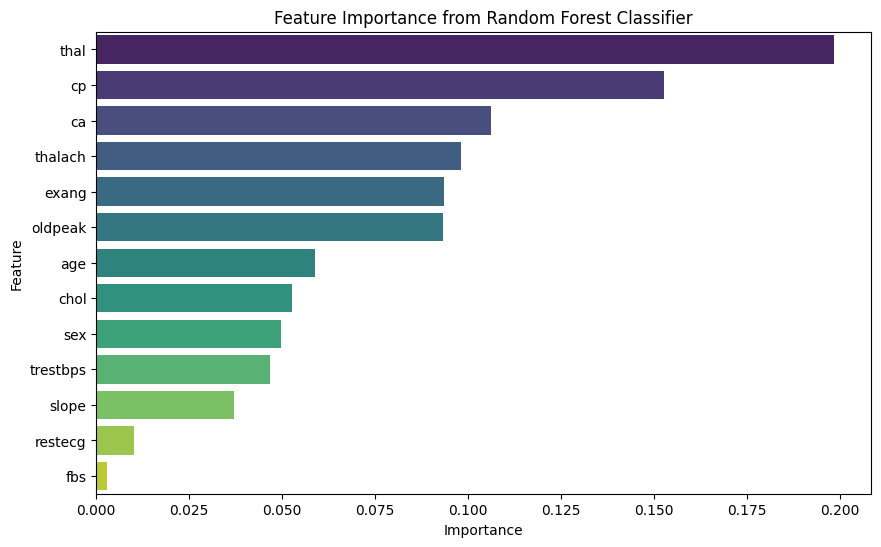
\includegraphics[keepaspectratio]{ans_files/figure-pdf/cell-15-output-4.png}}

The improved model is based on the original Decision Tree model with
SFS. The original Decision Tree has accuracy: 0.74 and sensitivity:
0.78, and the improved model has accuracy: 0.83 and sensitivity: 0.73.

\begin{enumerate}
\def\labelenumi{(\arabic{enumi})}
\setcounter{enumi}{15}
\tightlist
\item
\end{enumerate}

Contributions:

Yixin Ma: 11, 12, 13, 14, 15

Runhan Huang: 6, 7, 8, 9, 10

Kunhan Liang: 1, 2, 3, 4, 5, 15

\begin{enumerate}
\def\labelenumi{(\arabic{enumi})}
\setcounter{enumi}{16}
\tightlist
\item
\end{enumerate}

Link to the public repository: https://github.com/SweetIceLolly/3da-a6

\newpage

\section{References}\label{references}

GitHub Copilot was used as a code assistant for some of the questions.




\end{document}
